\documentclass{project}
\usepackage[pdfauthor={Morgan Jones},pdftitle={CS27510 Assignment},pdftex]{hyperref}
\usepackage{graphicx}
\usepackage{subcaption}
\usepackage{float}
\begin{document}
\title{CS27510 Assignment}
\subtitle{Student Information System}
\author{Morgan Jones (mwj7)}     
\version{1.0}
\status{Release}
\date{2016-04-23}
\maketitle
\tableofcontents
\newpage
\section{INTRODUCTION}
This report details a solution for a student information system designed to reduce workload on a summer school application company.  Currently all applications go through the application company and are forwarded manually to the summer camp leaders with the company responsible for getting extra applicant details to the schools after each of the applicants have been accepted.
\\\\
The company would like to have a website that enables the managing of applications and the application process to be done entirely by the individuals involved rather than all applications being directly reliant on the company. An ideal solution will be secure, robust and easy to use for both the applicants and the summer camp leaders. With the goal to minimize the time and effort spent by the company while facilitating the application process.
\\\\
This report lays out the requirements of such a system and presents the design and discussion of a back-end database and front-end web interface solution to be used by summer camp applicants and summer camp leaders during the application process. The choices of implementation are discussed and the design is detailed with references to provided visual representations of the web and database components of the system, these are included as appendices. Security, maintenance and disaster recovery are discussed and a conclusion is given summarizing the benefits of the overall system along with noting any issues or concerns.
\newpage
\section{FUNCTIONAL REQUIREMENTS}
This section details the functionality the final system will have.
\subsection{Interface requirements}
\begin{itemize}
\item The website must have a login/create new account page for users to access the site.
\item The website must reject any invalid input entered into forms by any users. 
\item Users must be alerted to any changes or errors that concern them.
\item Student users must be able to edit their profile information; camp leaders must be able to edit the information of their school.
\item Students must be able to use the website to list and search all summer camps registered.
\item Camp Leaders must be able to use the website to list and search any applications sent to their schools. 
\item All users must be able to view applications they send/receive. 
\item The site must contain help on how to use the site for it's users.
\item The site must contain contact details of the company for students and leaders to get in touch if they need.
\end{itemize}
\subsection{Business requirements}
\begin{itemize}
\item Anyone can create an account through the website as a potential summer camp applicant.
\item Employees in positions of leadership that work in any of the summer camps registered with the company can login to a leader's account.
\item Students must be able to write their applications on the website.
\item After acceptance or rejection an application status must change to alert the applicant. 
\item Upon acceptance applicants will be prompted to enter extra personal details.
\item There must be a deadline on the date at which a given summer camp is no longer taking applications.
\item There must be a deadline displayed for an applicant to respond if accepted.
\item There must be a link for students to pay for the summer camp through a third party once accepted and extra information has been entered.
\item Upon any student payment, transaction details must be kept and made available for proof or reference by the student making the payment. 
\item If a student applies for a summer school the same student cannot apply to that same summer school again.
\end{itemize}
\subsection{Security requirements}
\begin{itemize}
\item The only data available to someone not logged in should be that which is on the website homepage.
\item The website must reject any dangerous input entered into forms by users.
\item Students must not be able to edit any data other than their own information.
\item Students must not be able to read any information other than their own or that of the summer schools.
\item Leaders must not be able to edit any other information other than that of their own summer school.
\item Leaders must not be able to read any information other than the applications sent to them, the data of the students applying or there own schools details. 
\item Passwords and other sensitive information must not be human readable while stored in the database.
\item Password reset can be done securely through email if a student user's password is forgotten.
\end{itemize}
\newpage
\section{METHODS}
This section explains the reasoning and assumptions behind the major design choices of the system.
When designing the system I started with the database and focused on what data will be needed and how it will need to be structured, I then went about designing the web interface based off what access will be needed to the data and who will be accessing it. 
\\\\
I have chosen to have two tables for storing the users of the system, one for the students and one for the camp leaders, this is because the data that needs to be stored for the two types of users is very different. not all the users are in one place which may result in faster logging in because the amount of users needed to be searched is considerably less.
\\\\ 
I decided to introduce a summer schools table instead of hold summer school information in the summer camp leaders table to avoid repeating groups in the data (since each school can have more than one leader) thus making the database more normalised and wasting less space. The company makes it clear that students  apply to summer schools and not to summer school leaders therefore it only seemed right to have a separate database entity to represent the schools. In this initial design I have included the name of the school, cost of the course, the deadline for application and a short description as fields in the Summer Schools table because I have assumed that this information is needed to be displayed about each school for a student to identify it as one he/she would like to apply for.
\\\\
My design assumes that each summer school can have one-many camp leaders instead of exactly one because it is likely that more than one staff member working in a summer school will be responsible for applications. I made a choice between allocating each school a leader account and having the leaders of that school share the account, or allow multiple leader accounts to access to a schools profile as long as those leaders belonged to that school, I chose the latter.
\\\\
I have chosen to store for each school the deadline by which to apply and the number of days accepted students have to respond because of the logical assumption that the summer schools cannot take applications forever if the school course must start at some date in the future. 
\\\\
Different users have access to different functionalities and therefore different navigation bars, this makes the website easier to use by reminding users what they can do at all times.
Information on the website is expandable and searchable to allow users to view and edit the content they need with ease. All inputs are checked, any final decisions have confirm pop-ups and any changes or errors are made clear using alerts, this is so the user is aware at all times what he/she is doing.
\newpage
\section{RESULTS}
\subsection{Front end design}
This section details how the website front-end will be structured, what functionality each page will have and the interface each page provides to access that functionality.
These pages are represented in the figures in the Front end section of the appendices in this document. 
\begin{itemize}
\item \textbf{Homepage -}
The homepage~\ref{fig:homepage} will hold general information about the company, how to use the site and the company's contact details. This page, the create new account page and the forgotten password page are the only pages that users will not have to be logged in to view. From here a user can login~\ref{fig:homepage-login} using the 'Login' drop down.

\item \textbf{Create New Account Page -}
Here a user can create an account by entering a username and password, this page~\ref{fig:create-new-account} cannot be accessed if the user is already logged in. The password has to conform to the password security rules displayed on the page. Leaders accounts cannot be set up on the website, these will instead be pre-arranged between the summer schools and the company. Once a suitable password and username have been entered the user will be taken to their empty profile page to fill in the personal details required for the summer schools. After this the user will remain logged in.  

\item \textbf{Forgotten Password Page -}
This page~\ref{fig:forgot-password} allows a user to get an email sent to the email address on their profile with a link to reset their password. This page is used by students only and is accessed through the 'Forgot your password?' link in the login drop down on the navigation bar. 

\item \textbf{Reset Password Page -}
This page~\ref{fig:reset-password} can reset a student user's password. A student can only access this page through a link sent to them by email from the Forgotten Password Page. Once the user has entered an new valid password the password will be reset and the user taken to the Homepage to login using their new password.

\item \textbf{Student Profile Page -}
This page~\ref{fig:students-profile} holds all the student's basic information needed for application to summer school. The student can update this information at any time. For this information to be updated~\ref{fig:students-profile-good-input} each input box must have data of a valid type entered into i ~\ref{fig:students-profile-bad-input}. 

\item\textbf{Summer Schools Listing Page -}
This page~\ref{fig:summer-schools-listing} displays the summer schools registered with the company. The user can search through them or jump between pages of results. Each summer school has a small panel representing it, this displays the name of the summer school, its cost, the deadline by which to apply and a part of a short description of the school. A student user can select a school which will then take the user to a page where he/she can write to apply~\ref{fig:write-application}.

\item\textbf{Write Application Page -}
Here a prospective student can write his/her application and send it to a summer school. This page~\ref{fig:write-application} is displayed when a school from the schools list~\ref{fig:summer-schools-listing} is clicked by a student. The schools information is displayed on this page above a text area where the applicant can write an application to be sent by clicking the 'Submit Application' button.

\item\textbf{Student's Applications Page -}
This page~\ref{fig:students-applications},~\ref{fig:students-applications2} ,~\ref{fig:students-applications3} displays all the current student user's sent applications. Applications are either Accepted(Green), Pending(Orange) or Declined(Red) students can view or cancel ~\ref{fig:students-applications-remove} applications at any time from this page. When an application has been accepted the student can accept and pay for the course~\ref{fig:students-applications-confirmed} by using a link on this page added to the right of the application's title. 

\item\textbf{Transaction History Page -}
This page~\ref{fig:transaction-history} displays all a student user's transaction details from any previous payments made for summer school.

\item\textbf{Student Transaction Page -}
Here~\ref{fig:student-transaction} a student can enter passport information for the summer school and  payment details for later reference, once this data has been entered the user can click a link to the third party site to pay for summer school course.

\item\textbf{Summer School Profile Page -}
Here~\ref{fig:school-profile} the leader account used by the summer school can change the cost,description, deadline of the application and the amount of days after acceptance students have to accept. The data saved on this page is the information prospective students will see when searching through the Summer Schools Listings Page.

\item\textbf{Leader's Applications Page -}
Here~\ref{fig:leaders-applications},~\ref{fig:leaders-applications2} a summer school leader can manage his/her received applications. There is a tab for unevaluated, accepted and declined applications because of the volume of applications received; there is also a search box to easily find applications in each tab. A Leader can accept or decline an unevaluated application at any time from this page as well as see the profile details of students that have sent applications to the leader's school.
\end{itemize}
There is a navigation bar that is persistent throughout the pages once a user is logged in; there is a different navigation bar depending on if the user is a student, summer camp leader or not yet logged in. 
\begin{itemize}
\item \textbf{When logged in as a student user} the navigation  bar has links to the Homepage,  Summer School Listings Page, Student's Applications Page, Student Profile Page and a logout link that will log the user out and return them to the company Homepage.

\item \textbf{When logged in as a summer camp leader user} the navigation bar has links to the Homepage,  Leader's Applications Page, Summer School Profile Page and a logout link that will log the user out and return them to the company Homepage.

\item \textbf{When not logged} in the navigation bar has links to the Homepage, Create New Account Page and a log in pop-up which is used for users to login, when using this to log in to a leader account the 'Log In As Leader' check box must be ticked.
\end{itemize}
On every page that takes user input there will be alerts displayed upon submission, informing the user of the quality of the input entered, these alerts are similar to the ones on the student profile page~\ref{fig:students-profile-good-input},~\ref{fig:students-profile-bad-input}. Confirm dialogues similar to the one shown on the student's applications page~\ref{fig:students-applications-remove} will occur every time the user attempts to make a final decision. 
\clearpage
\subsection{Database design}
This section details how the database tables are used, who uses them and how they are linked. These tables are represented as the figures~\ref{fig:conceptual-database-model},~\ref{fig:logical-database-model},~\ref{fig:physical-database-model} in the Database Design section of the appendices in this document. 
\begin{itemize}
\item\textbf{Student Applicants Table - }
Holds all the students personal information needed for summer camp application. The data in this table is entered and updated by the individual students with the exception of the username, password hash and password salt that are stored for authorization purposes. 

\item\textbf{Camp Leaders Table -}
Holds the login details of the camp leaders. No information is needed about camp leaders therefore this table only holds usernames, hashed passwords and password salts. This table is linked to the Summer Schools table since each leader account belongs to exactly one summer school. The information isn't read or edited by anyone and is only used for authorization upon login.

\item\textbf{Applications Table -}
Holds all the written applications. Many students can apply to many schools therefore this table is a link table between the Students and Summer Schools tables. The status and text of the applications are stored in this table with the IDs of the students and schools the application concerns. Entries in this table can be removed by the student to whom they belong at any time.

\item\textbf{Transactions Table -}
Holds transaction details about the payments made to the summer camps by the students. Linked to the student table because a student could have made zero or more transactions. A student can read (but not edit) their transactions from this table at any time through the website. 

\item\textbf{Summer Schools Table -}
Holds data about all summer schools registered with the company. There is a link between this table and the Camp Leaders table because each school has one or many leaders there is also a link between this table and the applications table because a school can have zero or more applications. Any of the camp leaders can change the details stored in this table about his/her school at any time. 
\end{itemize}
The basic queries needed to retrieve/update groups of data for particular users from the above tables will be written into the database as stored procedures instead of programmed into the website application's code slightly reducing how the coupling between database and the web interface. 
\newpage
\subsection{RDBMS and front end design platform}
The database will be implemented in PostgreSQL and the web interface will be written using PHP on the server-side and a JavaScript on the client-side.
\\\\
PostgreSQL:
\begin{itemize}
\item Will save the company money because it is a free-to-use database.
\item Has implicit locking to be used in preventing concurrency issues when multiple users try to manipulate the same data.
\item Supports table partitioning allowing for better query performance, this would be very useful for the company's large database.
\end{itemize}
For the front end PHP is a good choice because it is widely used and has many powerful libraries and functions that will make a lot of our website functionality easier to build, such as:
\begin{itemize}
\item A mail function that can be used to send emails to users for password reset.
\item Powerful encryption and hashing functions to be used on sensitive information before storing it.
\item Functions for sanitizing input from the user on the server-side. 
\end{itemize}
\subsection{Security} 
My design implements most of its security at the application level using usernames and passwords for authentication and authorization, a password must conform to the rules shown on the Create New Account page.
\\\\
Before storage each password will be prepended with a salt, this salt will be generated using a Cryptographically secure pseudo-random number generator (function available in PHP). The combination of the salt and the password will then be hashed with a standard sever side hash function. Hashing is necessary to prevent the passwords being seen if anyone had permission to read or managed to get hold of the databases data. The addition of a random salt to passwords prevents the same password being hashed in the same way, thus removing the possibility of an attacker using lookup tables, reverse lookup tables, or rainbow tables to gain access to user passwords.
\\\\
Password hashes, password salts and usernames will be stored in the database in the users table. To validate a user on login the user's salt and hash will be retrieved from the database. The salt will be prepended to the provided password and then hashed using the same hash function. If the resulting hash matches that stored in the database then the password is correct and the user is logged in.
\\\\
There will be a new random salt for every password to prevent a duplicate salt occurring , meaning if a user were to reset his/her password or create a new account then a new salt would have to be generated.
\\\\
All user input through the website will be sanitized and validated on the client-side through JavaScript and on the server-side through PHP. Sanitization and validation will be done on the client side to increase performance by reducing the amount of data being sent between the client and server every time incorrect input is entered. Sanitization and validation will be done on the server for security purposes refusing malicious or incorrect input regardless of what the client sends to the server.
\\\\
Data will be implicitly locked by the database for concurrency control.
\newpage
\subsection{Maintenance and disaster recovery}
\subsubsection{Maintenance}
\begin{itemize}
\item Preventive maintenance must be carried out in the form of routine backups and in the case of a database failure data will need to be recovered.
\item If the system needs to expand its functionality then extra entities and attributes may need to be added. 
\item If a summer school wants to create an account or remove one then, as my design states, the company staff will have to manipulate the data themselves to do this. 
\item Stored procedures and/or views to retrieve frequently needed information may have to be written.
\item The staff users will have to be assigned access permissions which will have to be maintained.
\end{itemize}
\subsubsection{Disaster recovery}
Database failures are impossible to prevent therefore this section out lines the design for backups and recovery.
\\\\
The Database files and log files, files that record all changes made to the database, will have off-site back up copies. The database will use archive logging when recording database changes to prevent any transactions being overwritten and lost.
\\\\
To keep the system on-line and available to the company's large amount of customers
incremental hot backups will be made. This means the database will remain on-line while all changed data and newly generated log files are copied to the back up location. This may degrade performance slightly but the system is still accessible to the users, the backup isn't copying the complete database meaning it will take less time to complete.
\\\\
When recovering the database will use the log files to rollback/rollforward transactions, this is a better alternative to manually reprocessing the data because the system stores a large amount of data.
\newpage
\section{DISCUSSION}
This section discusses some possible issues with the designed system.
\\\\
My design allows students to confirm attendance with more than one summer school. It could be argued that the system should not allow this because it goes against the logic of the business seeing as no student can attend two summer schools at once. If I were to expand my database design to include the start and end dates of the summer schools the website could stop students to applying for schools whose dates overlap the dates of the school the student is currently confirmed a place at.
\\\\
Everything in the business process after the payment to the summer school is outside the scope of this system. My design will assume summer schools will keep in contact using email or other methods once they have a confirmed student. Including a more detailed section on the application process is recommended as part of the information to be put on the Homepage.
\\\\
Every leader from one summer school has access to all that school's applications and profile information therefore one leader might be able to accept an application and another leader from the same school could reject it. I justify this in my design by assuming it's the responsibility of the individual summer camps to look after the accounts they request from the company and only allow trusted staff access to those accounts.
\\\\
My design does not cover the way in-which leaders create accounts; for my design to work summer camp leaders will have to independently contact the company to arrange the creation of a leader account. The company staff will have to update the database to add leader accounts for the summer schools this will be an extra responsibility of the staff which may not be ideal for the company.  
\newpage
\section{CONCLUSION}
Overall the system I designed is easy to use, always online and provides the company's customers with straight forward control over the data they need whenever they need it.
Implemented back end with a powerful free-to-use RDBMS, the solution is secure in how it stores and allows access to its data. Performance has been considered throughout the design process from the way the tables are structured and data is backed up to the way that input is validated between the client and server.
\\\\
From working on this report I have gained an awareness of the range of possibilities and benefits available for implementing logic at the database level when designing a database orientated solution.
I have learnt what needs to be considered when designing the procedure for a systems backup and recovery.  
\newpage
\section{APPENDICES}
\appendix
\subsection{Front end design}
\begin{figure}[H]
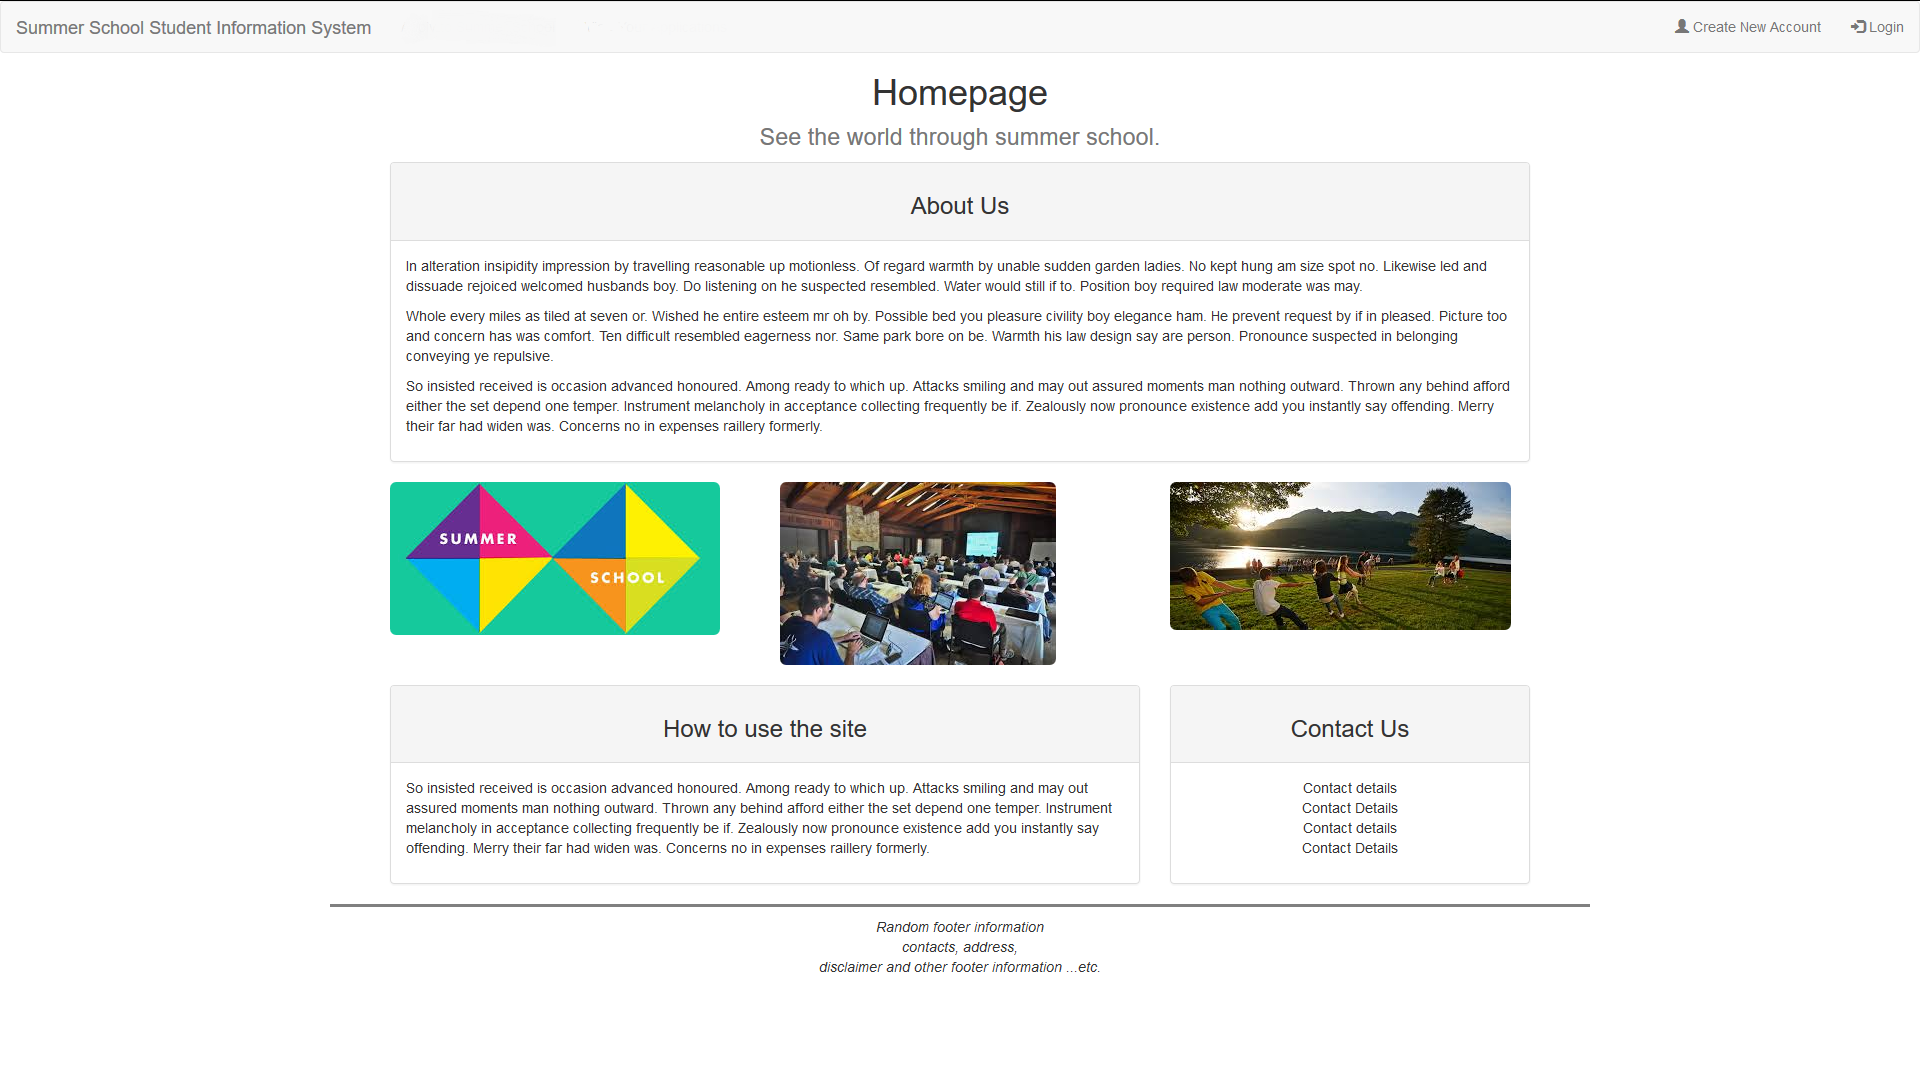
\includegraphics[width=\linewidth]{homepage.png}
\caption{Homepage}
\label{fig:homepage}
\end{figure}
\begin{figure}[H]
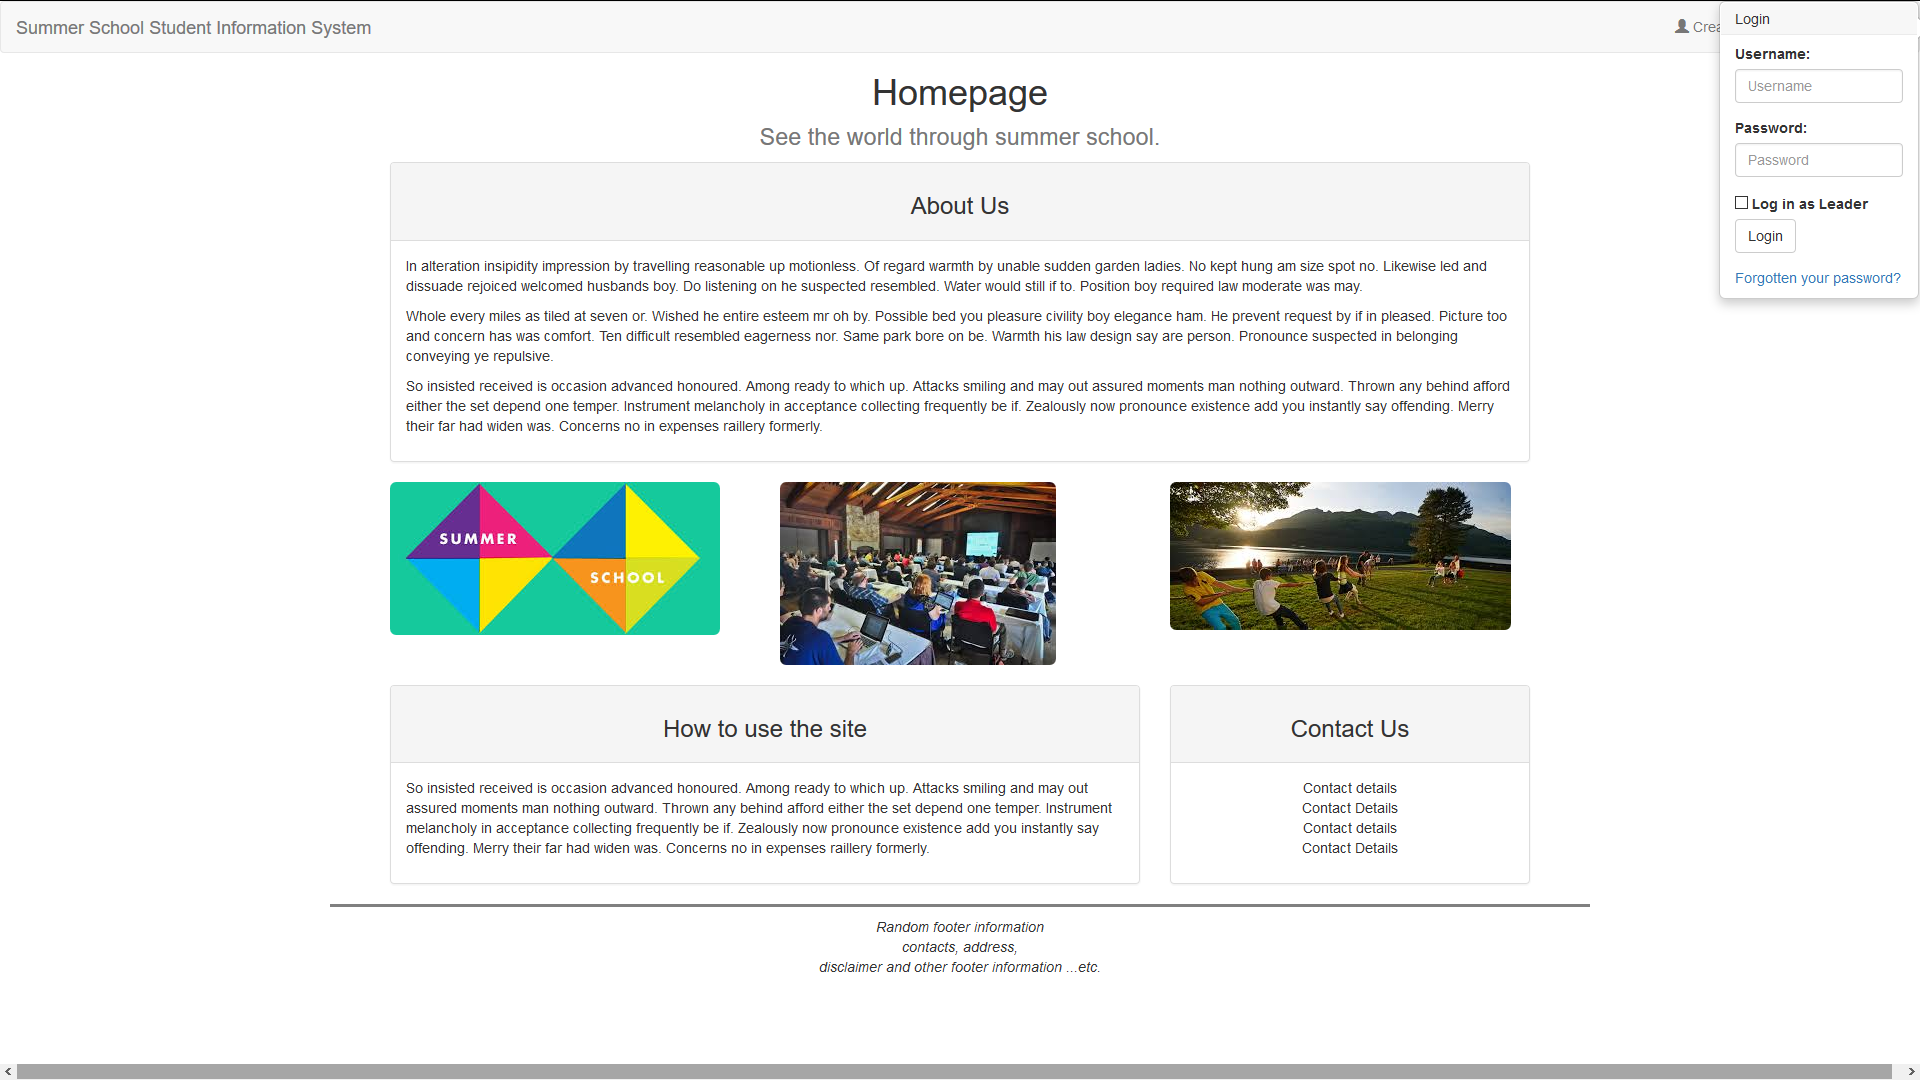
\includegraphics[width=\linewidth]{homepage-login.png}
\caption{Homepage - Login}
\label{fig:homepage-login}
\end{figure}
\begin{figure}[h]
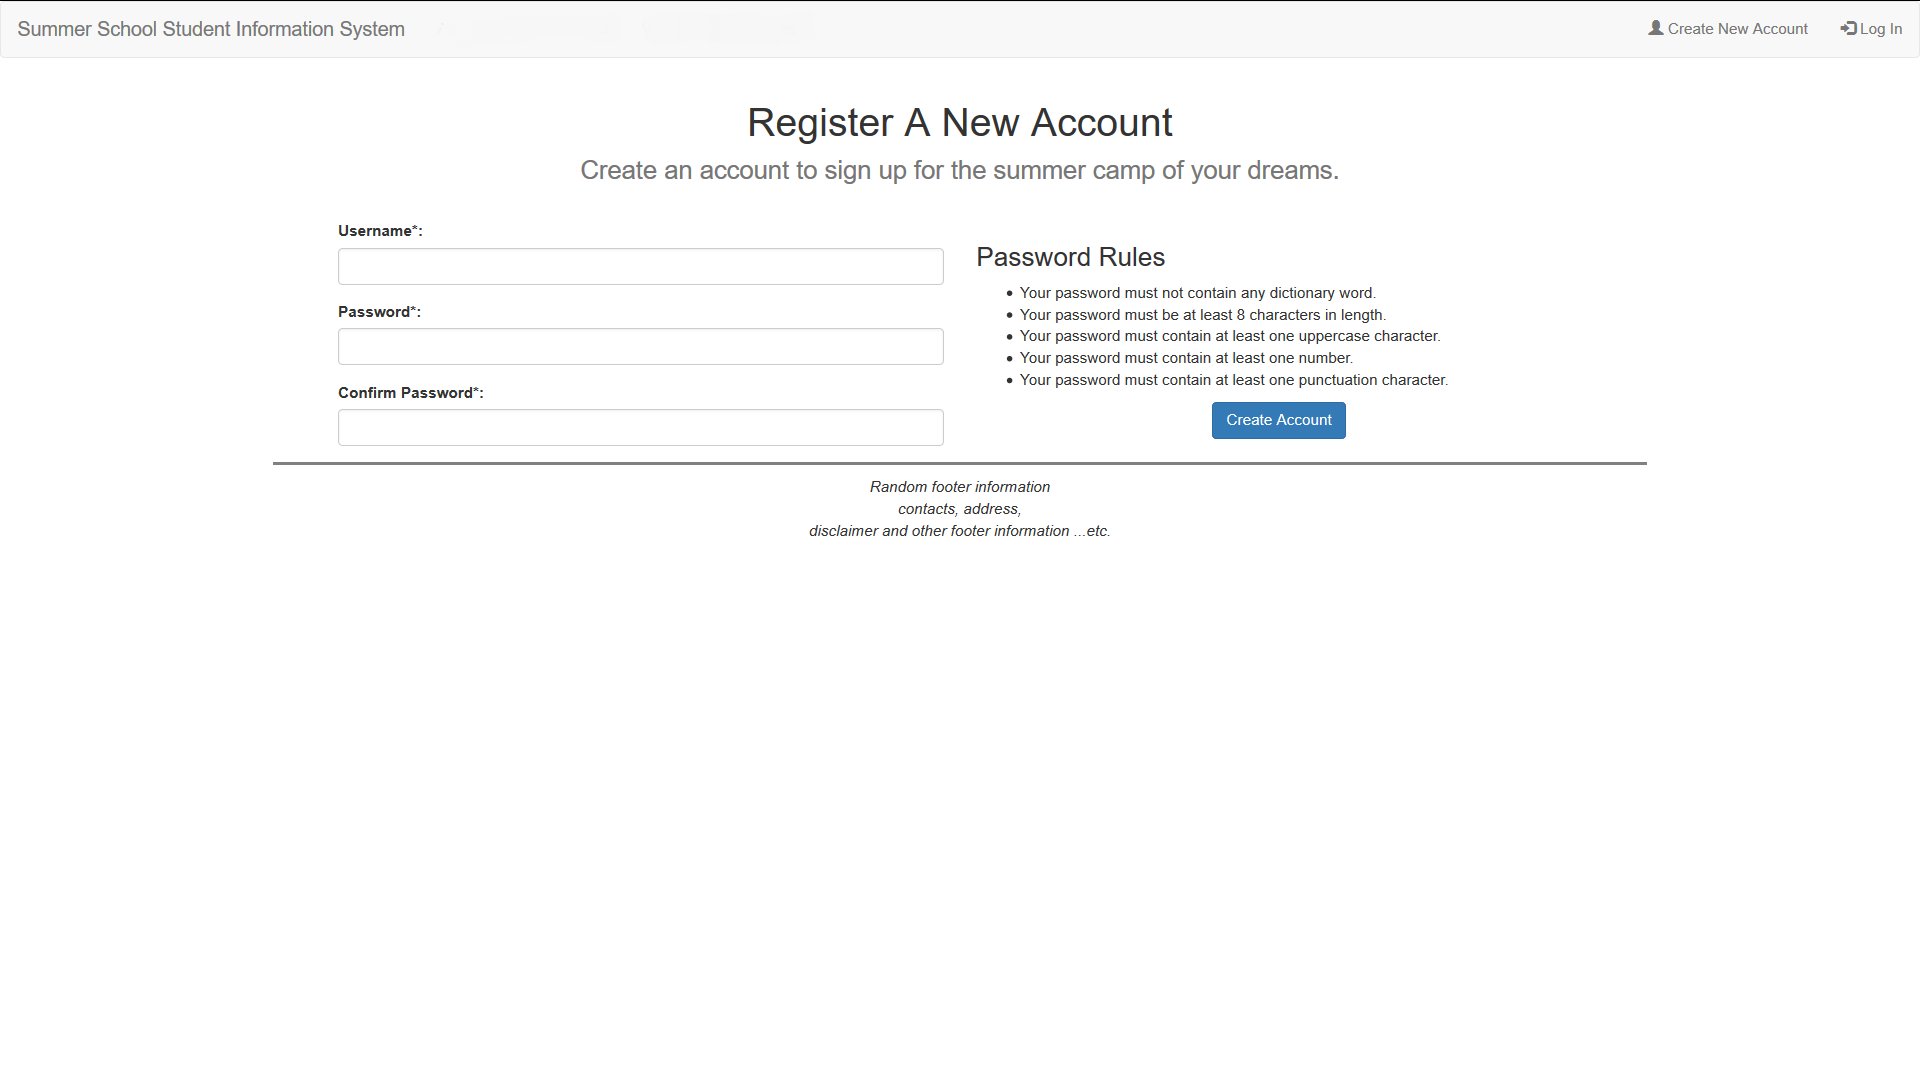
\includegraphics[width=\linewidth]{new-account.png}
\caption{Create New Account Page}
\label{fig:create-new-account}
\end{figure}
\begin{figure}[h]
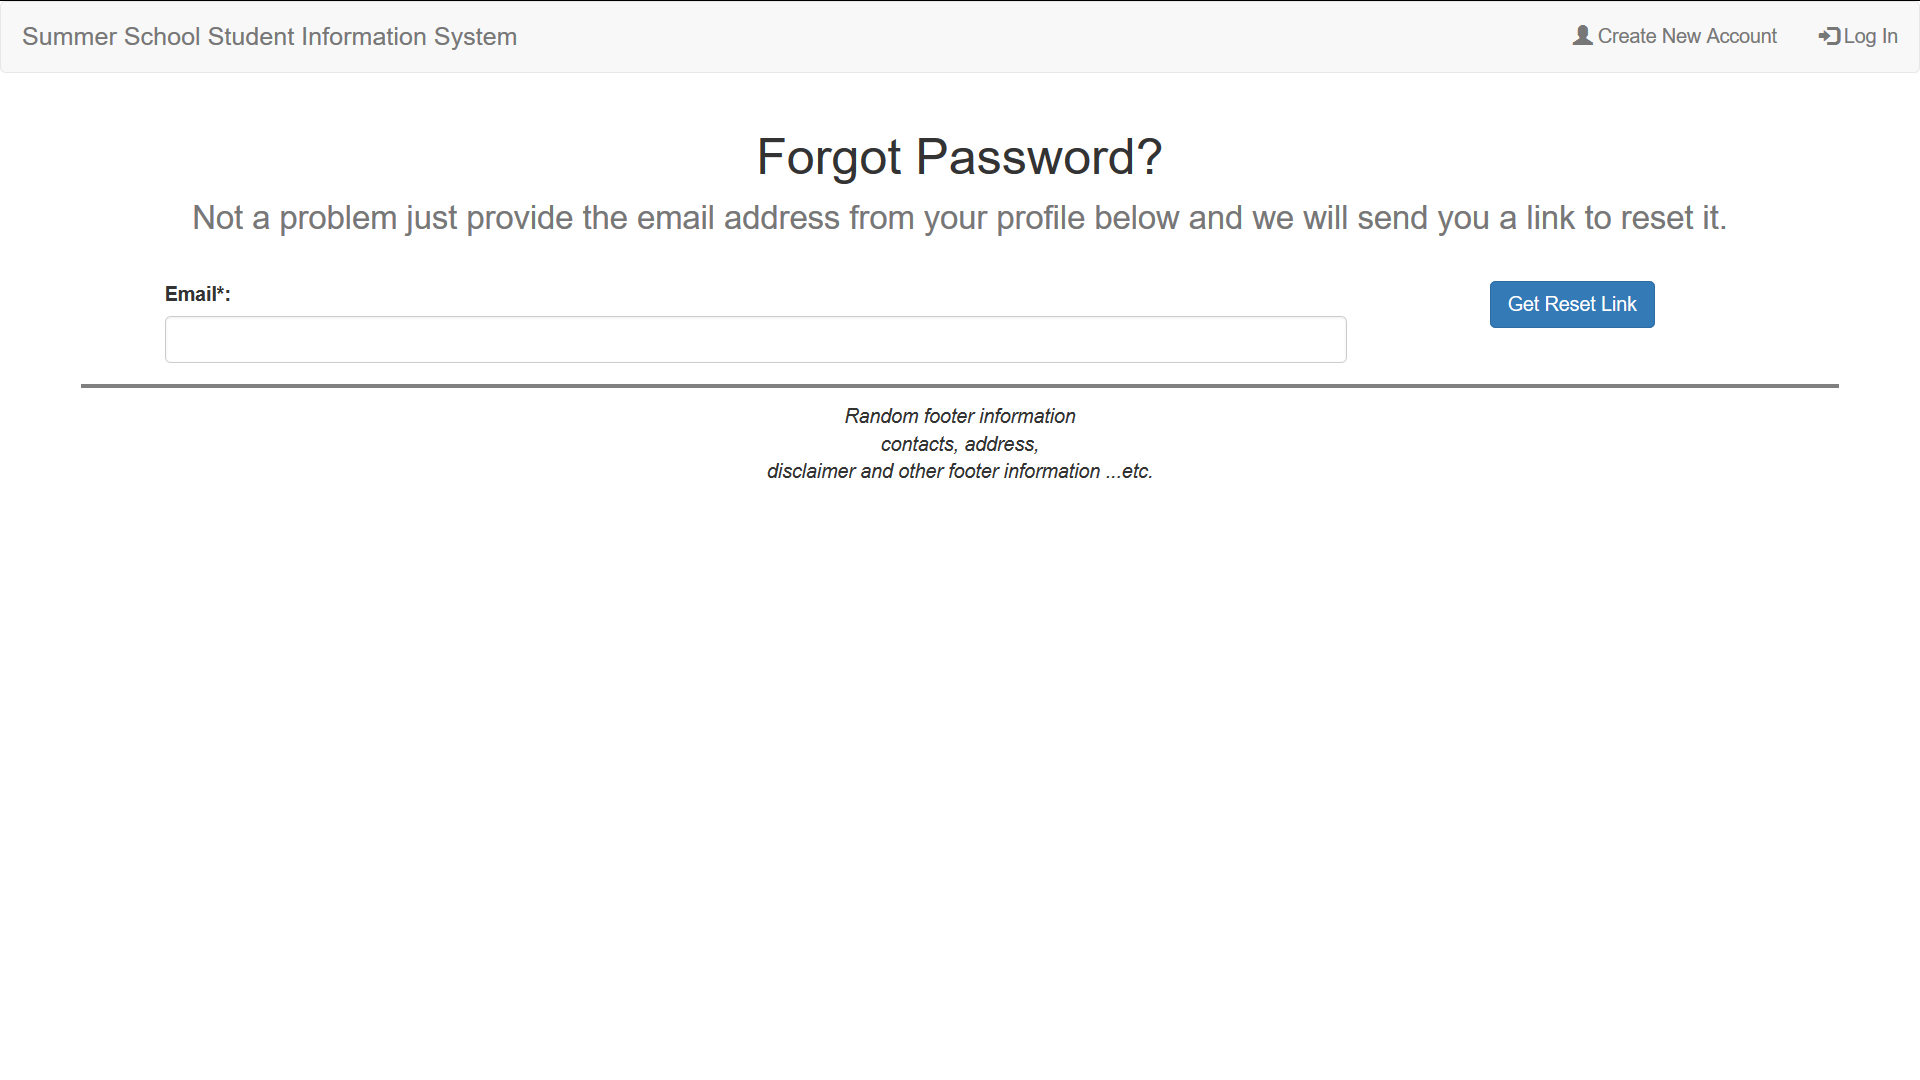
\includegraphics[width=\linewidth]{password-forget.png}
\caption{Forgotten Password Page}
\label{fig:forgot-password}
\end{figure}
\begin{figure}[h]
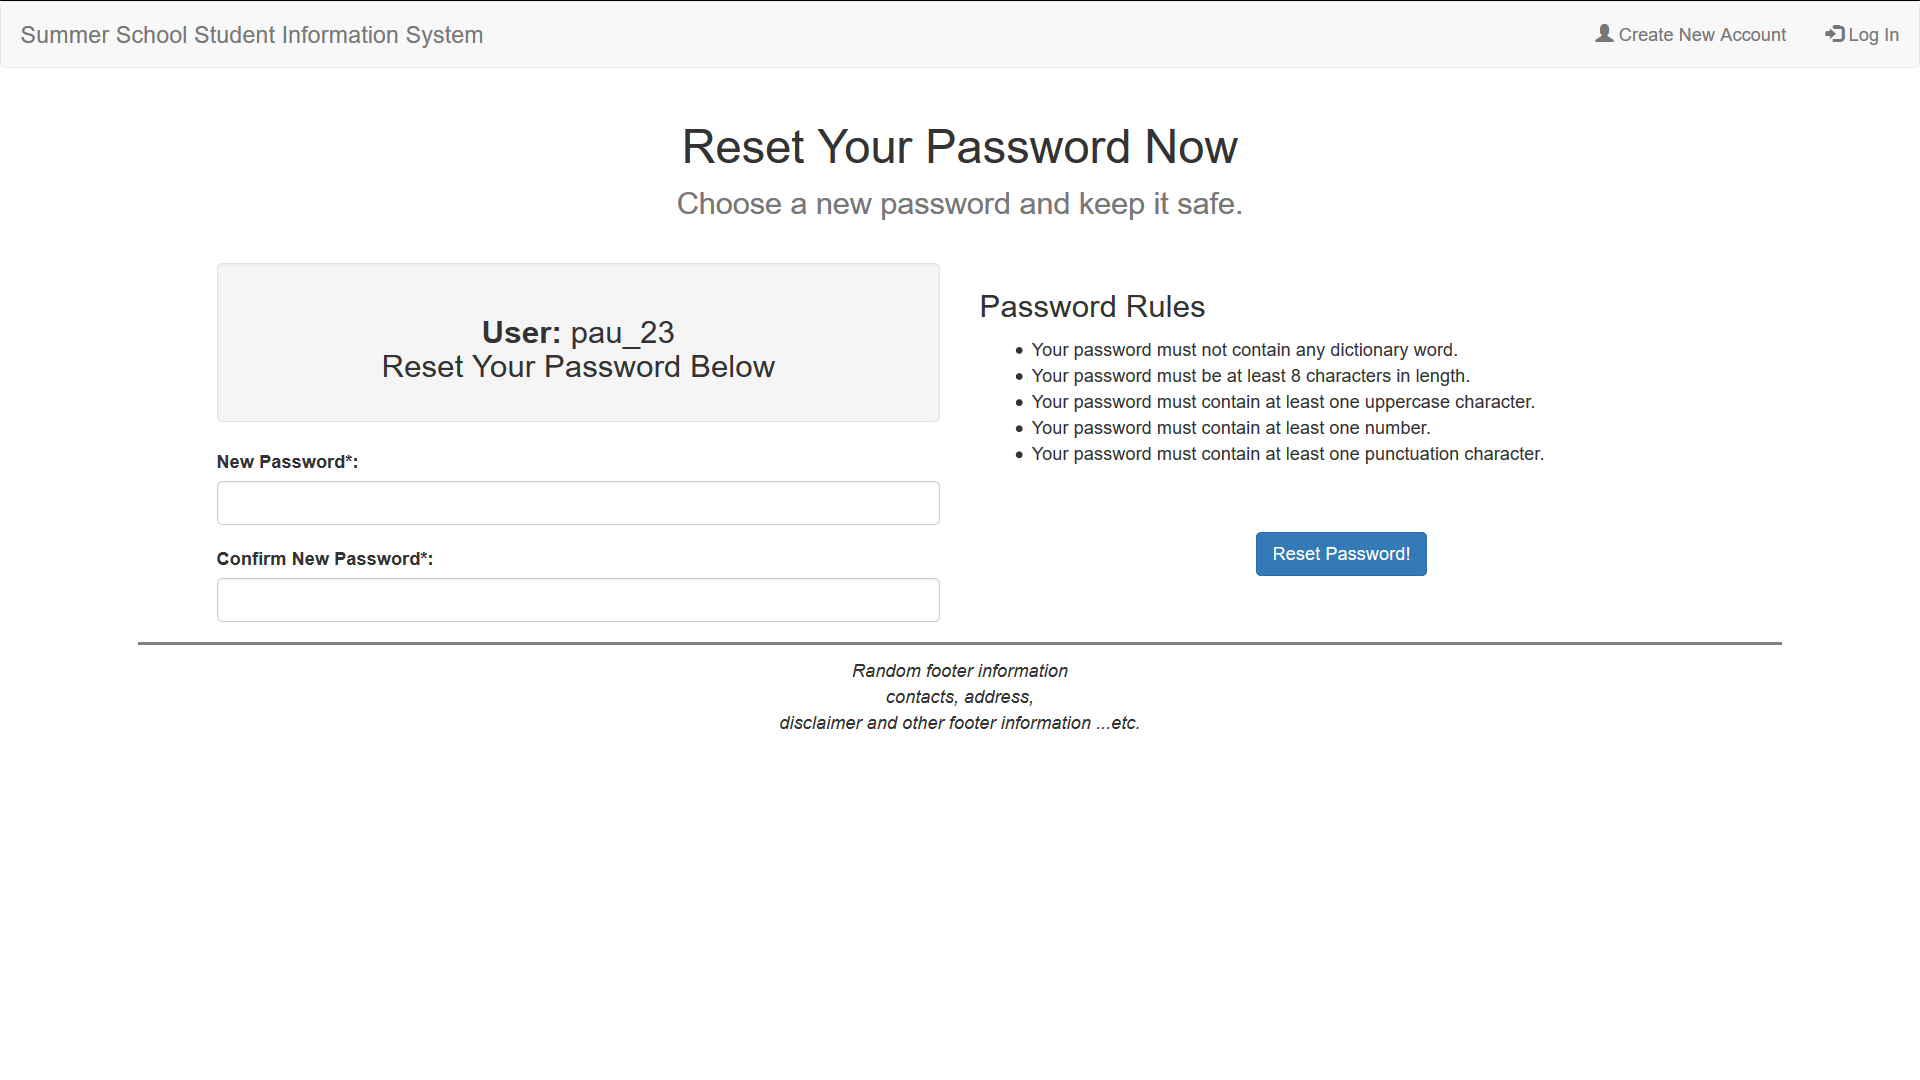
\includegraphics[width=\linewidth]{password-reset.png}
\caption{Reset Password Page}
\label{fig:reset-password}
\end{figure}
\begin{figure}[h]
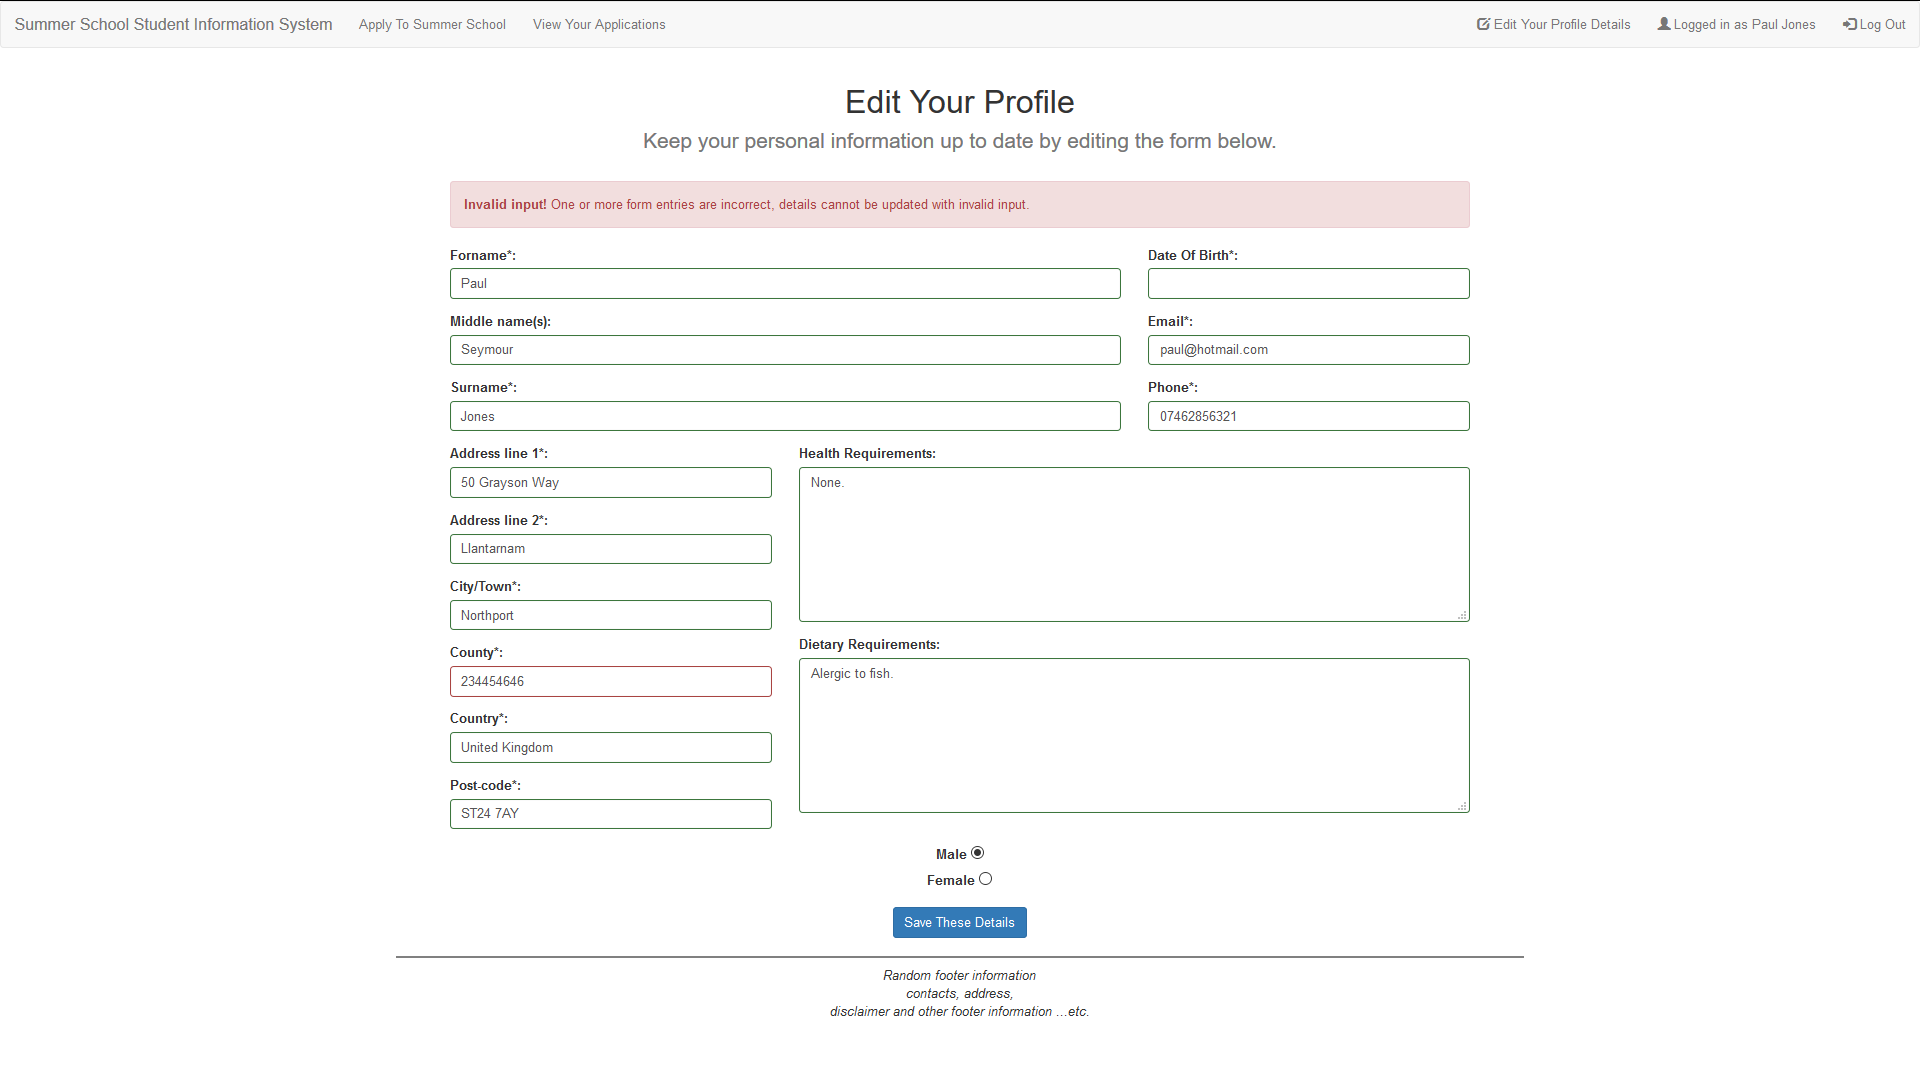
\includegraphics[width=\linewidth]{profile-edit-incorrect.png}
\caption{Student's Profile Page - Invalid Input Not Saved}
\label{fig:students-profile-bad-input}
\end{figure}
\begin{figure}[h]
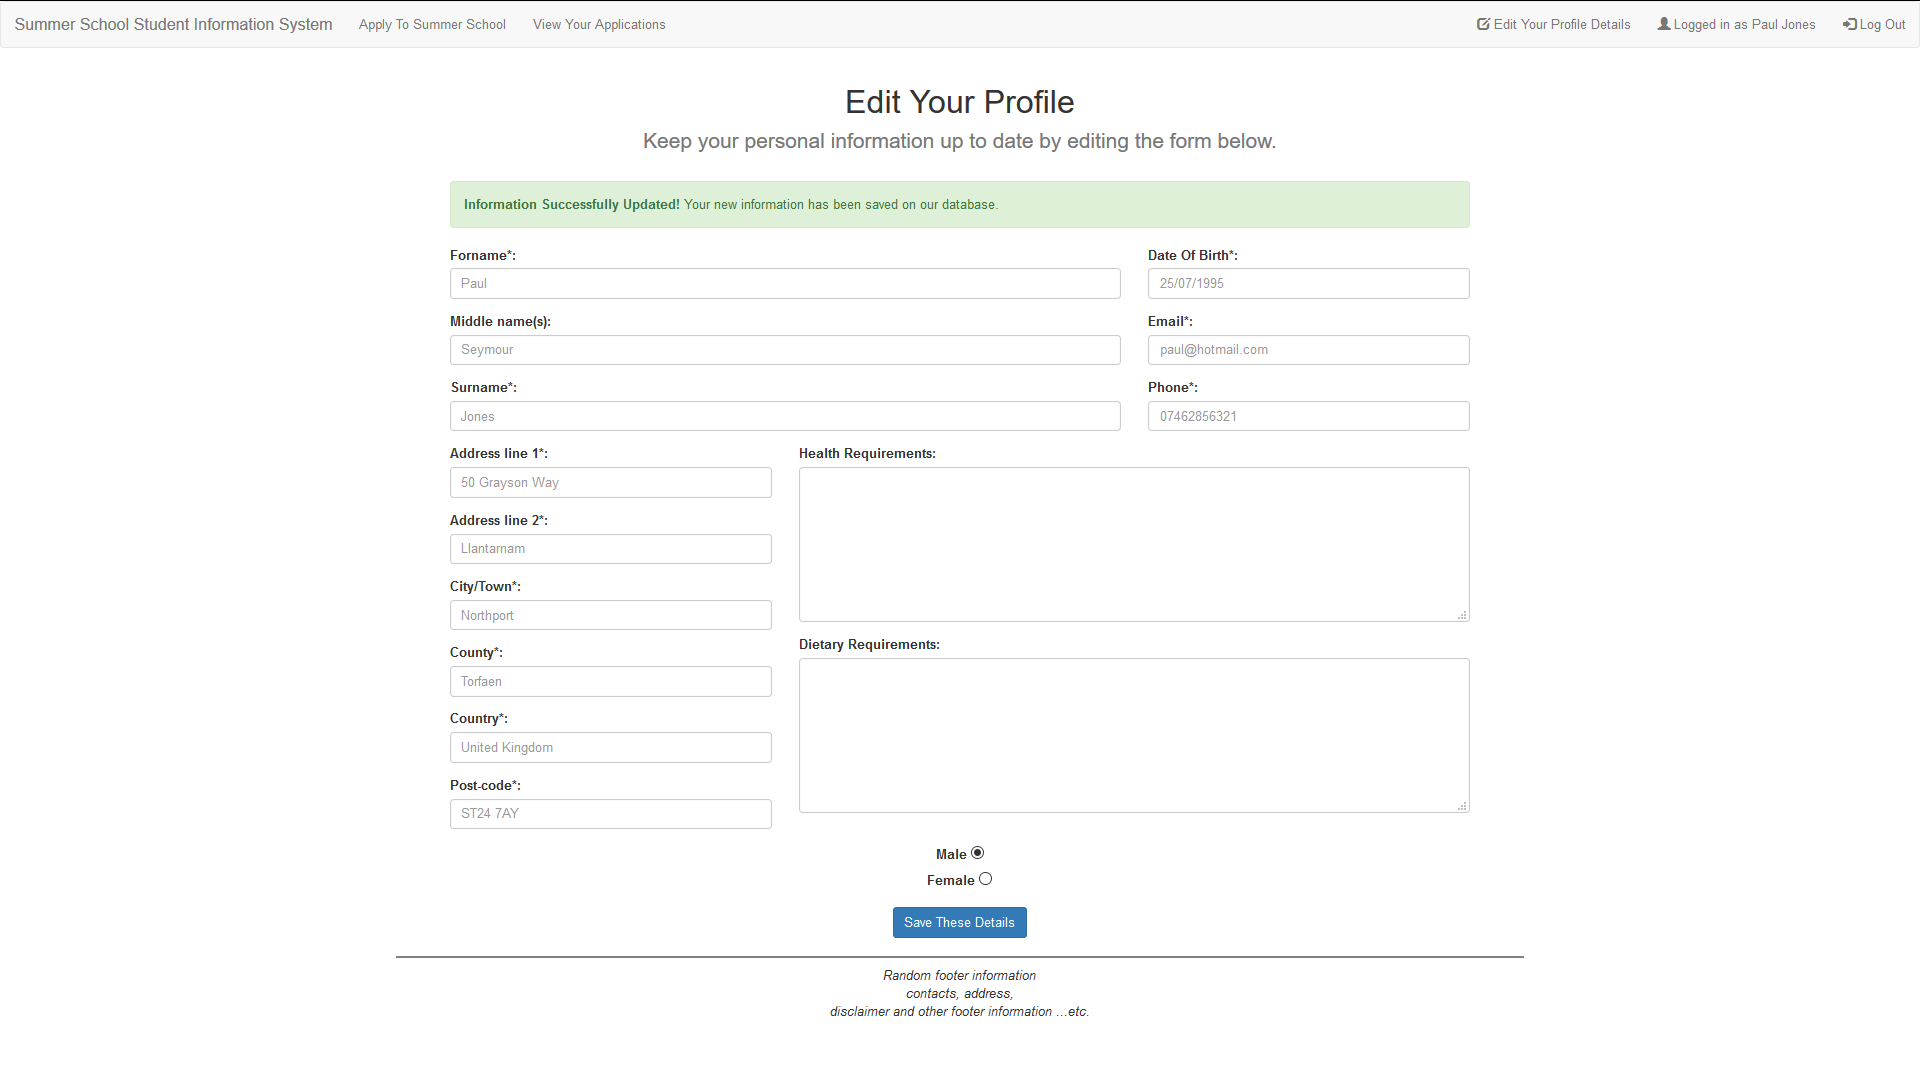
\includegraphics[width=\linewidth]{profile-edit-correct.png}
\caption{Student's Profile Page - Correct Input Saved}
\label{fig:students-profile-good-input}
\end{figure}
\begin{figure}[h]
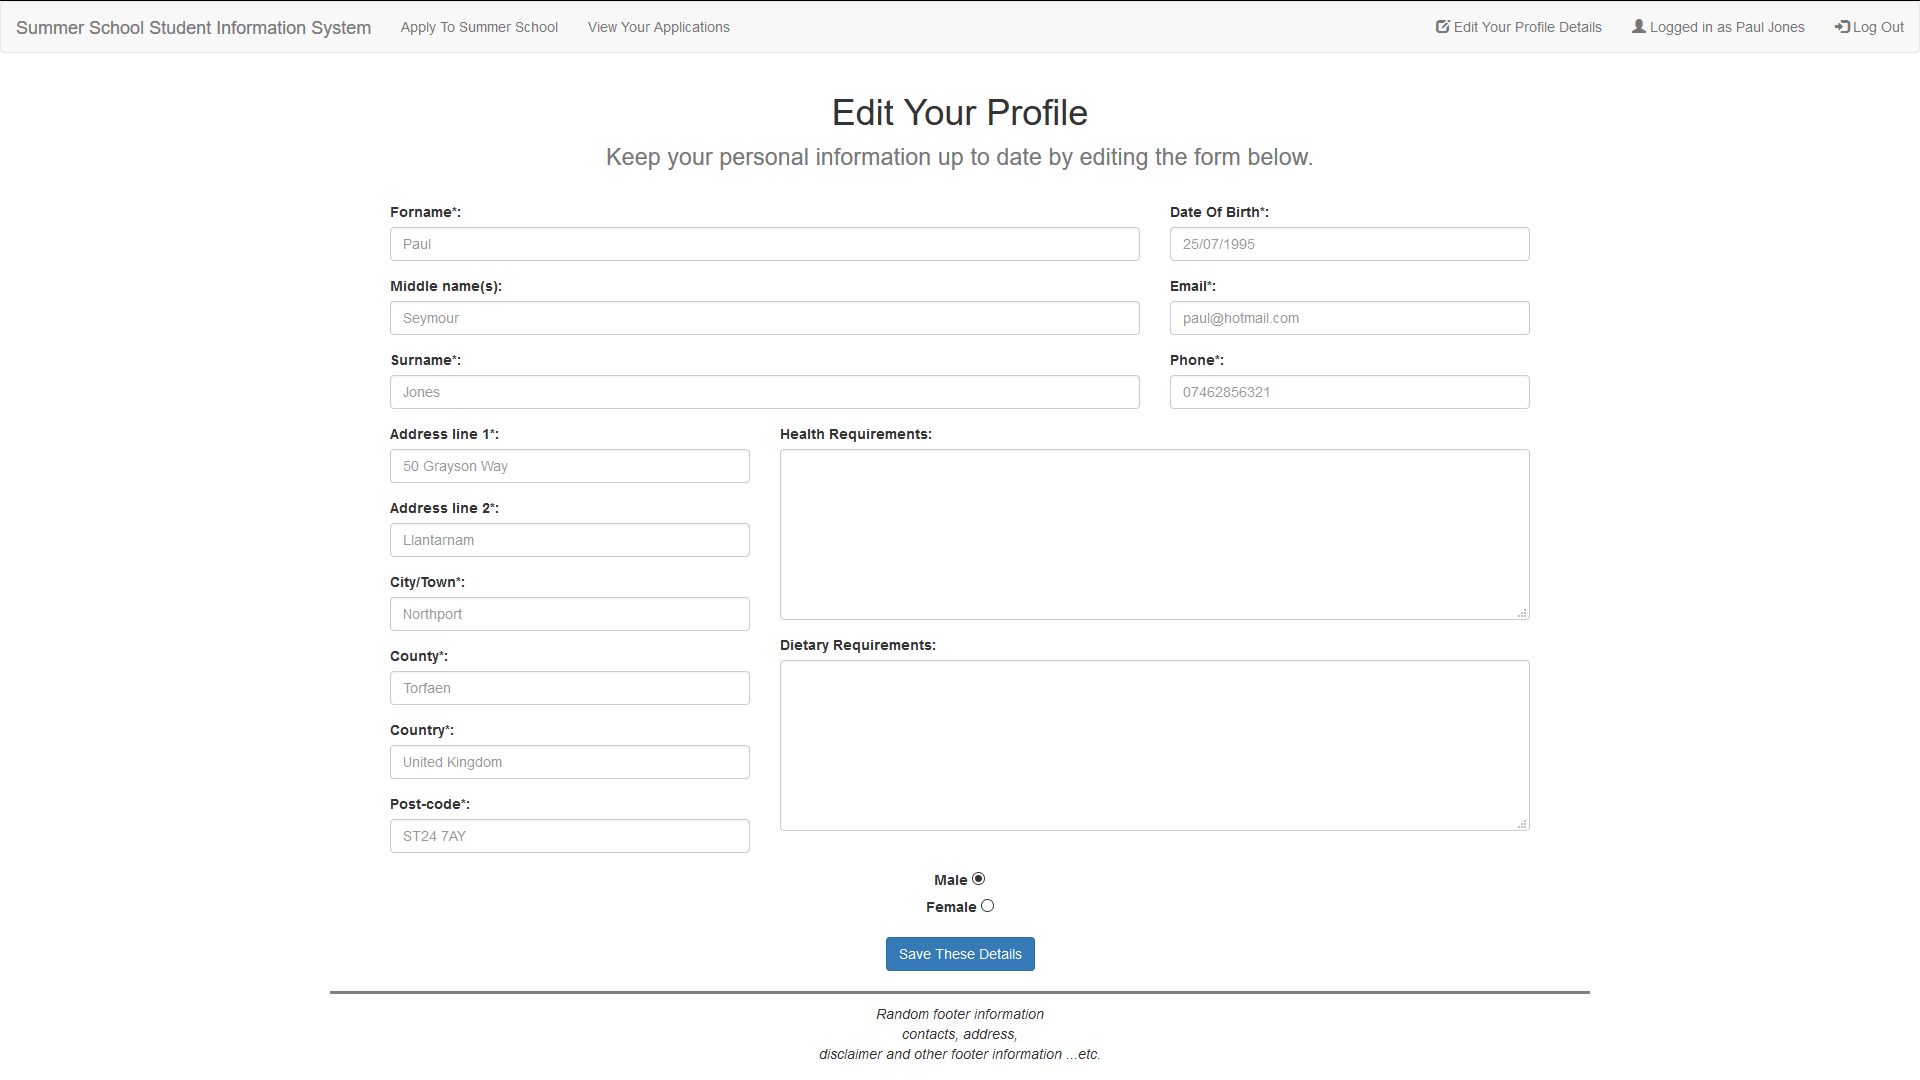
\includegraphics[width=\linewidth]{profile-view.png}
\caption{Student's Profile Page}
\label{fig:students-profile}
\end{figure}
\begin{figure}[h]
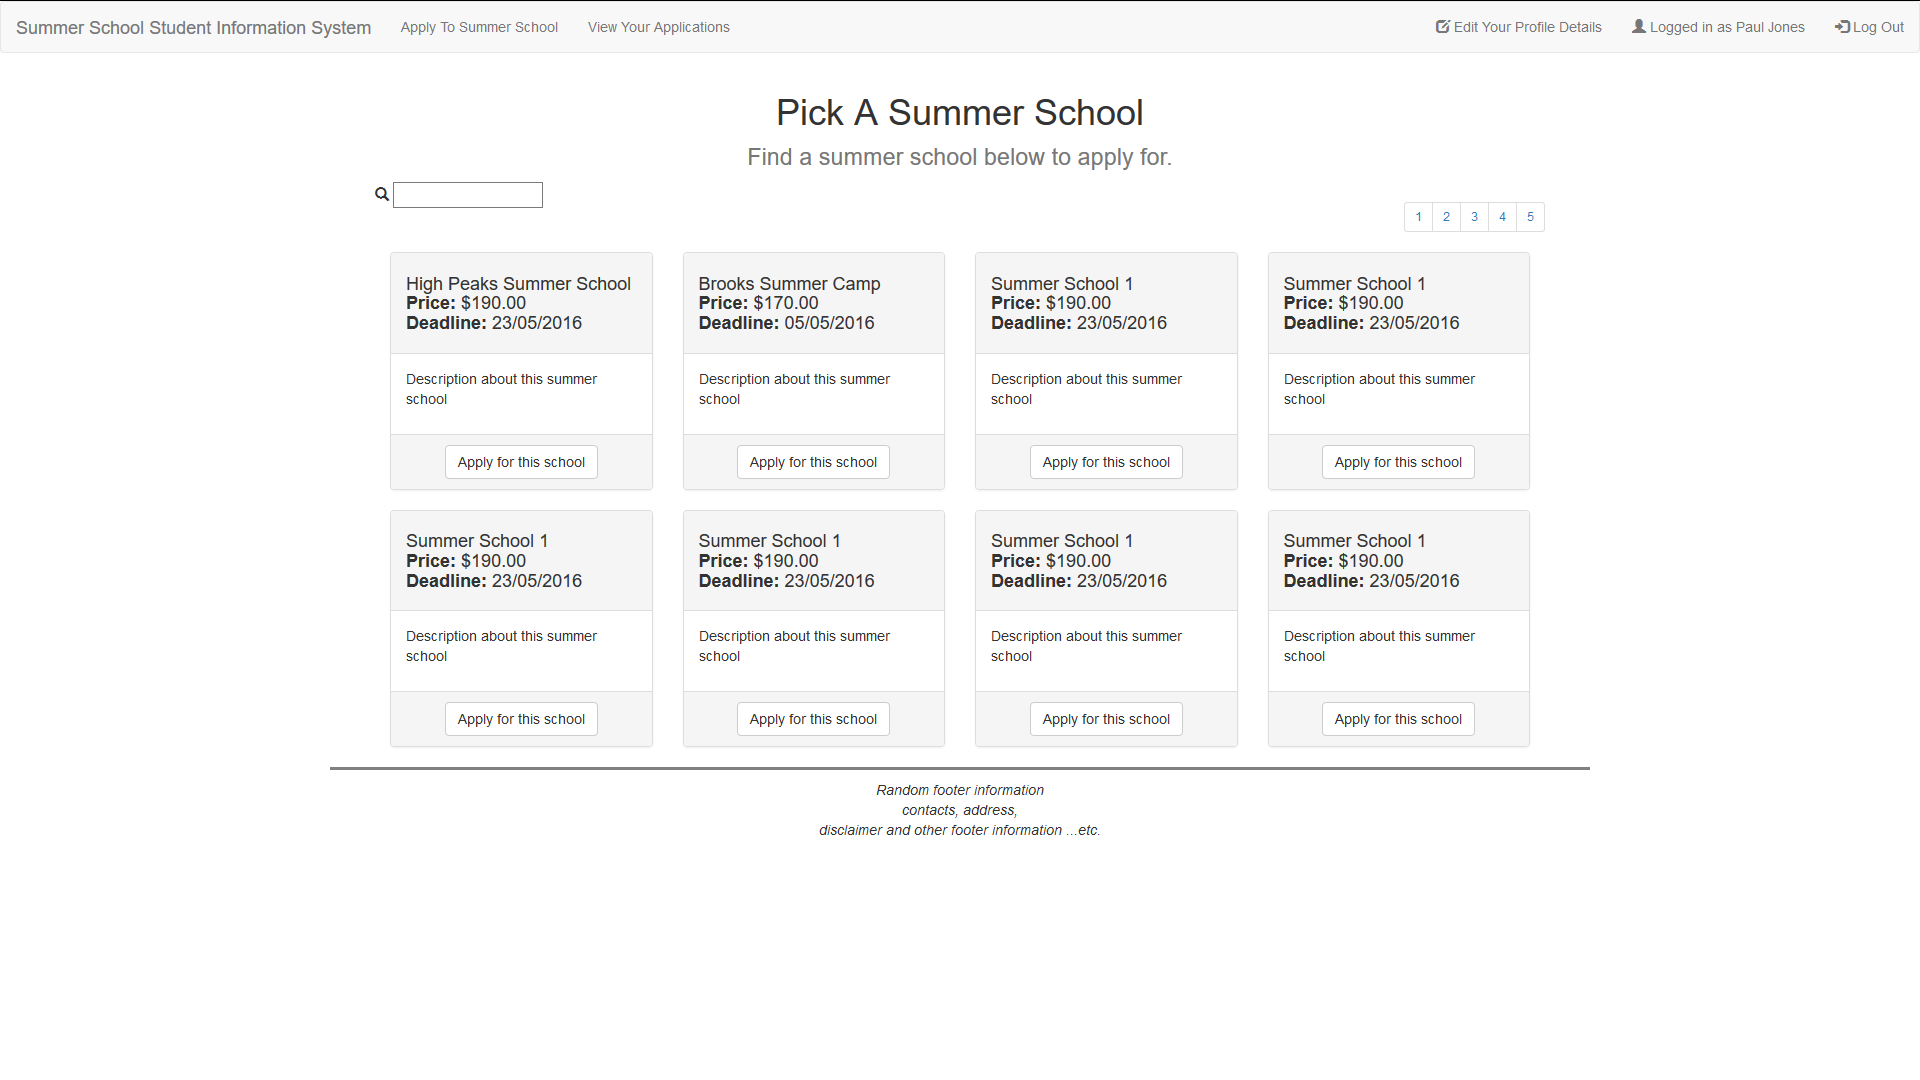
\includegraphics[width=\linewidth]{schools.png}
\caption{Summer Schools Listing Page}
\label{fig:summer-schools-listing}
\end{figure}
\begin{figure}[h]
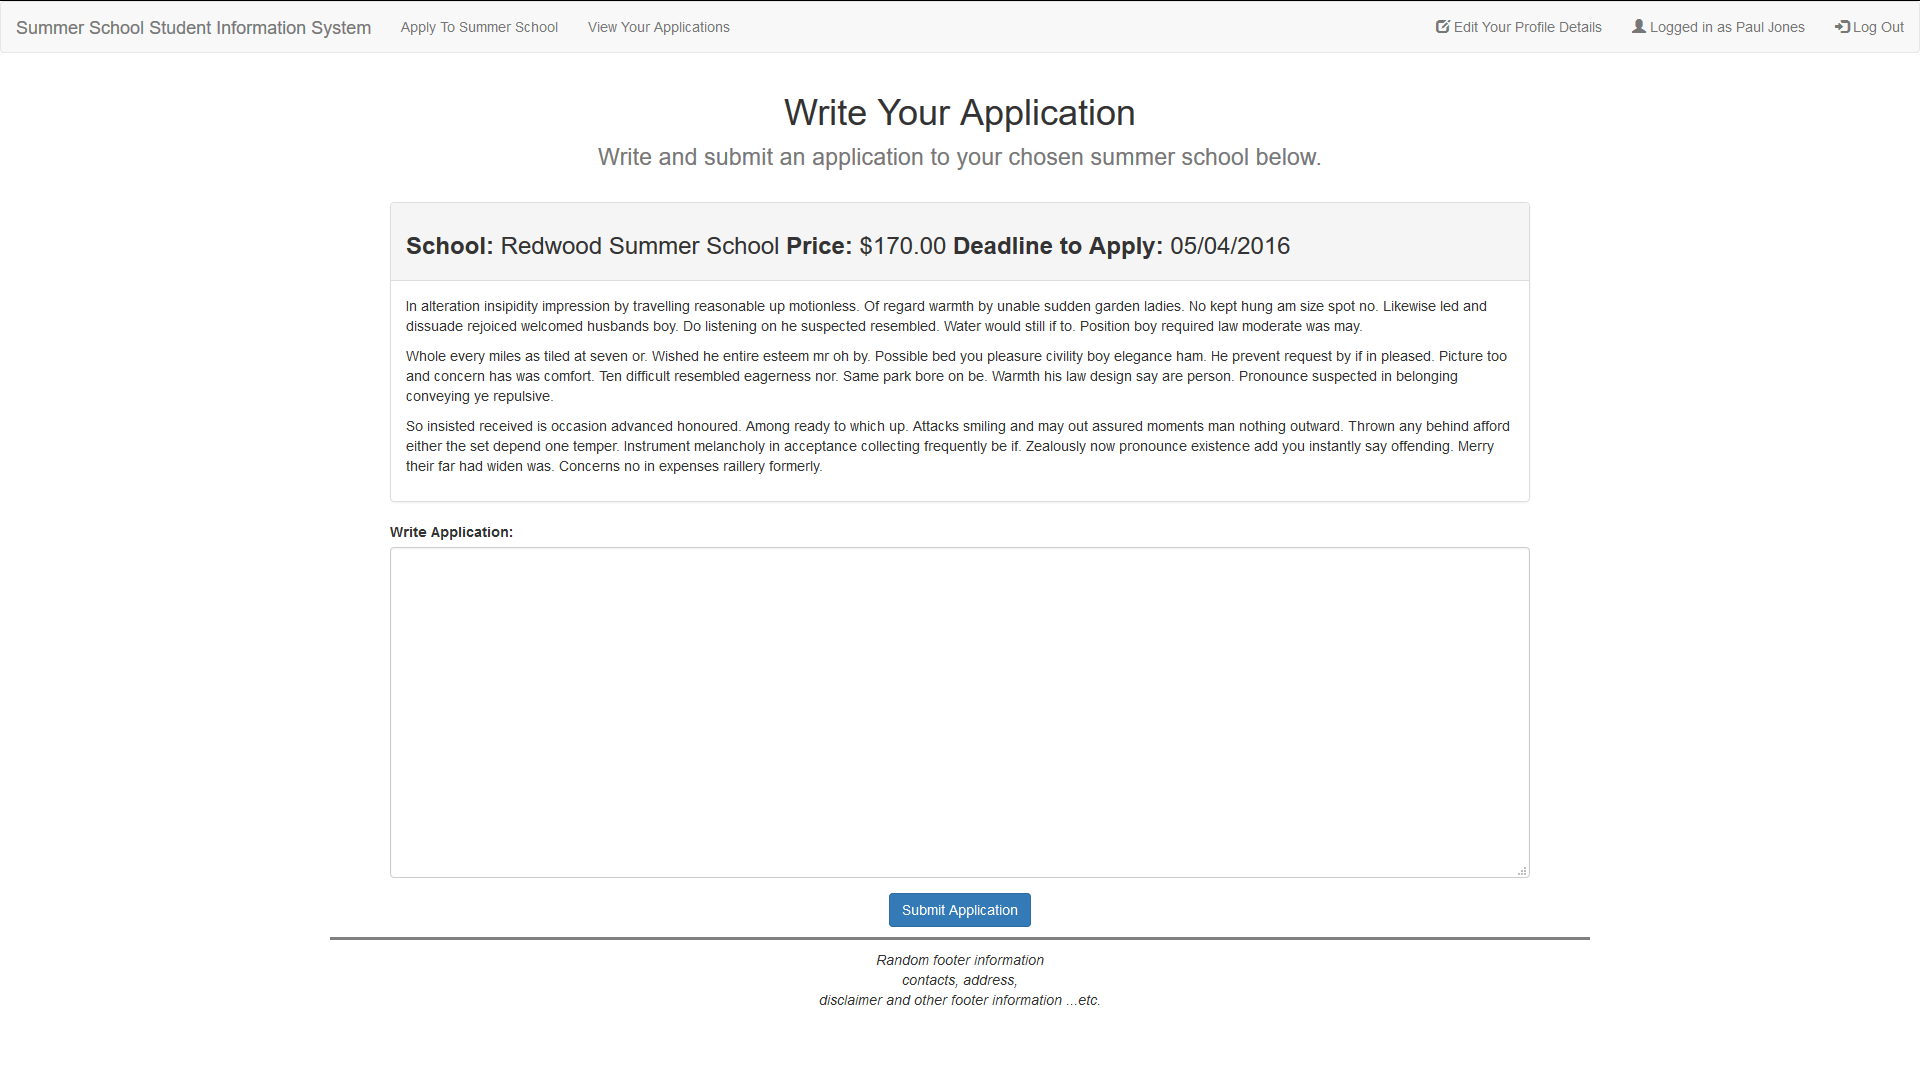
\includegraphics[width=\linewidth]{apply.png}
\caption{Write Application Page}
\label{fig:write-application}
\end{figure}
\begin{figure}[h]
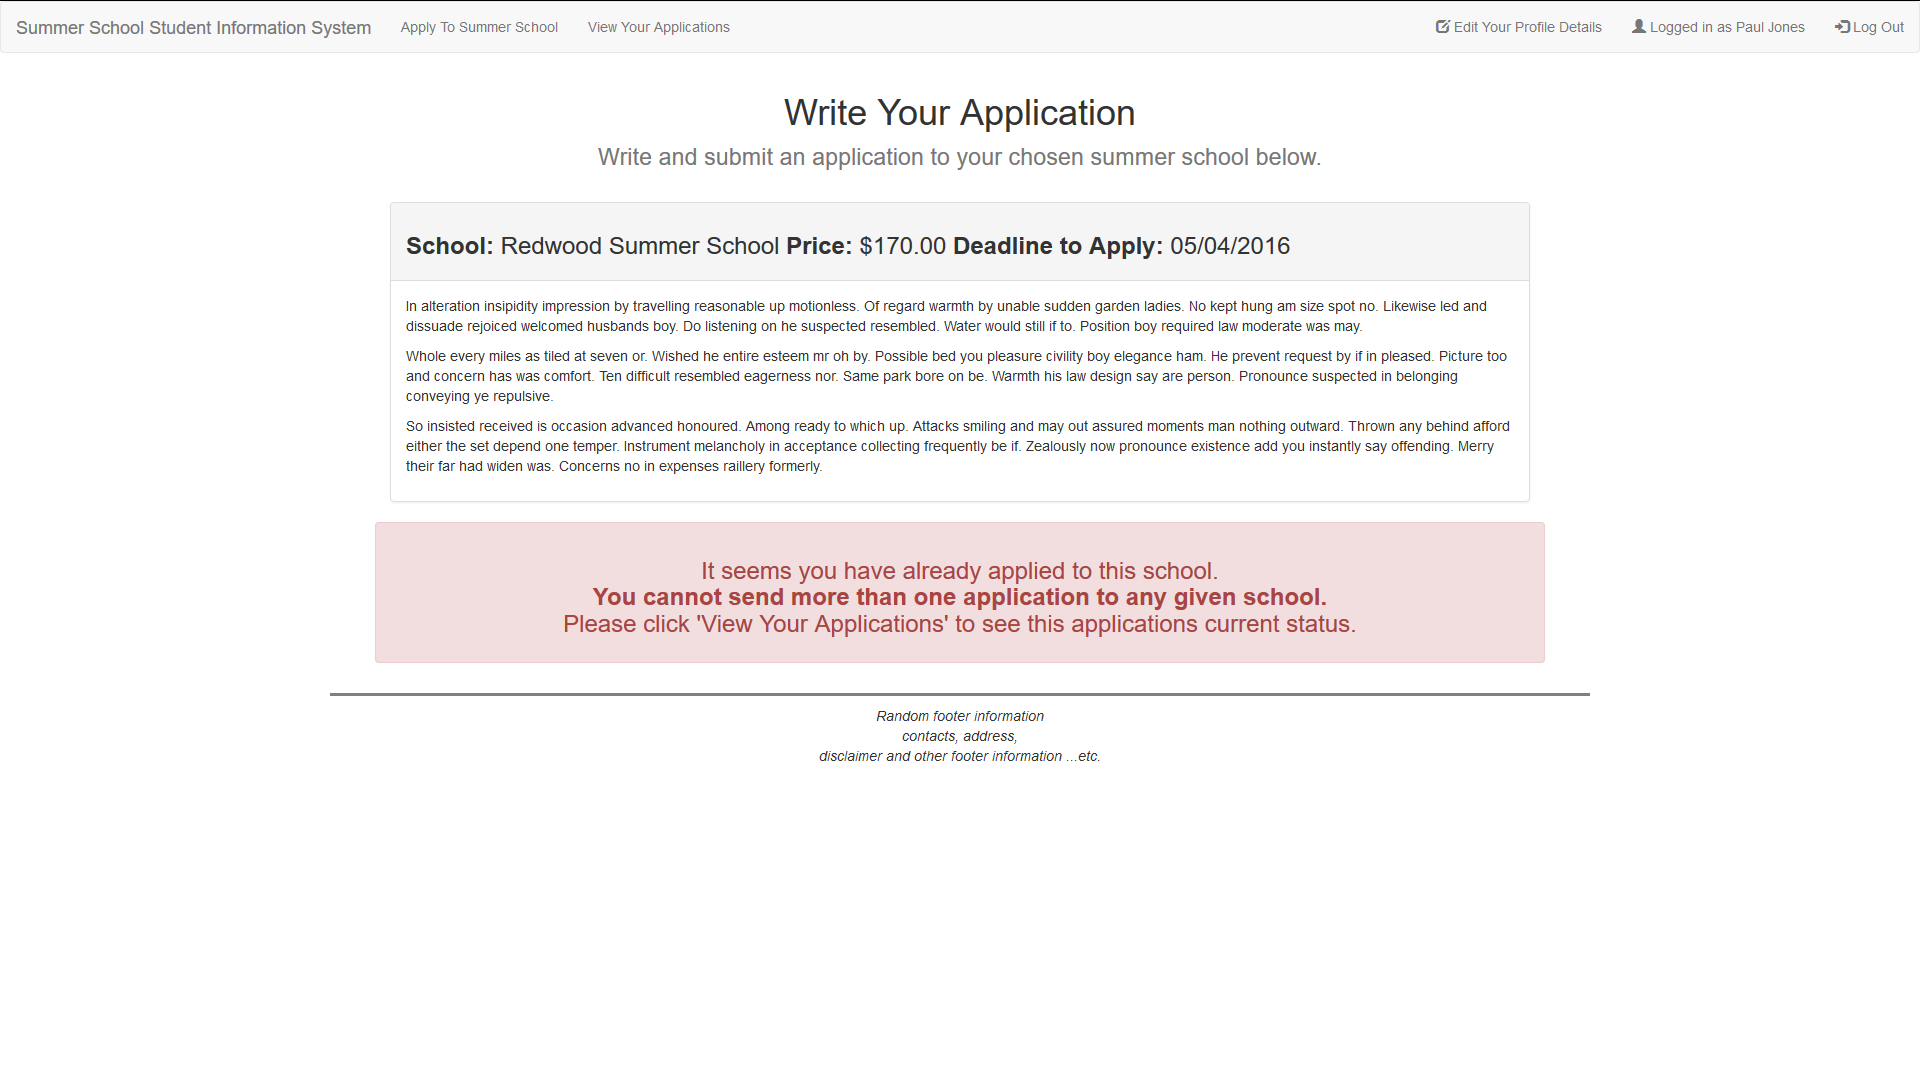
\includegraphics[width=\linewidth]{apply-fail.png}
\caption{Write Application Page - Reject attempt to apply to same school again}
\label{fig:write-application-reject}
\end{figure}
\begin{figure}[h]
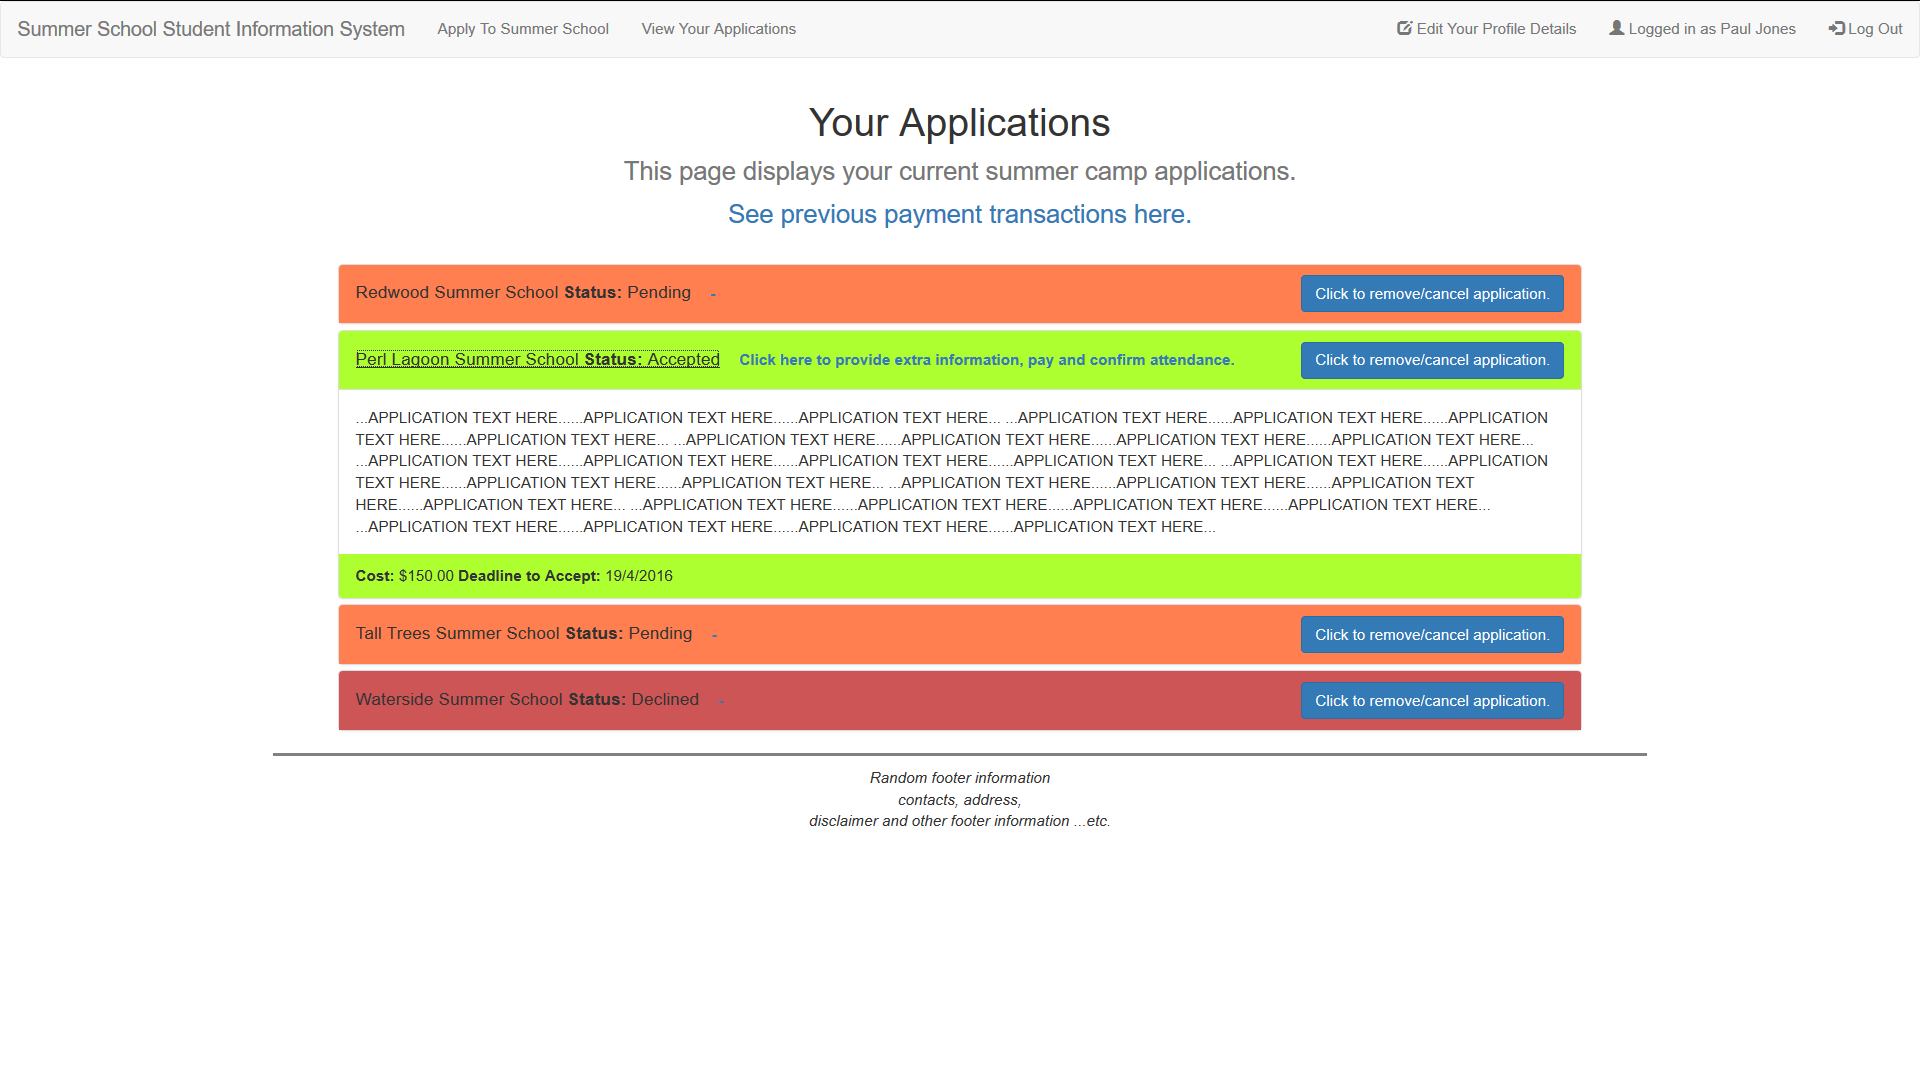
\includegraphics[width=\linewidth]{student-app.png}
\caption{Student's Applications Page}
\label{fig:students-applications}
\end{figure}
\begin{figure}[h]
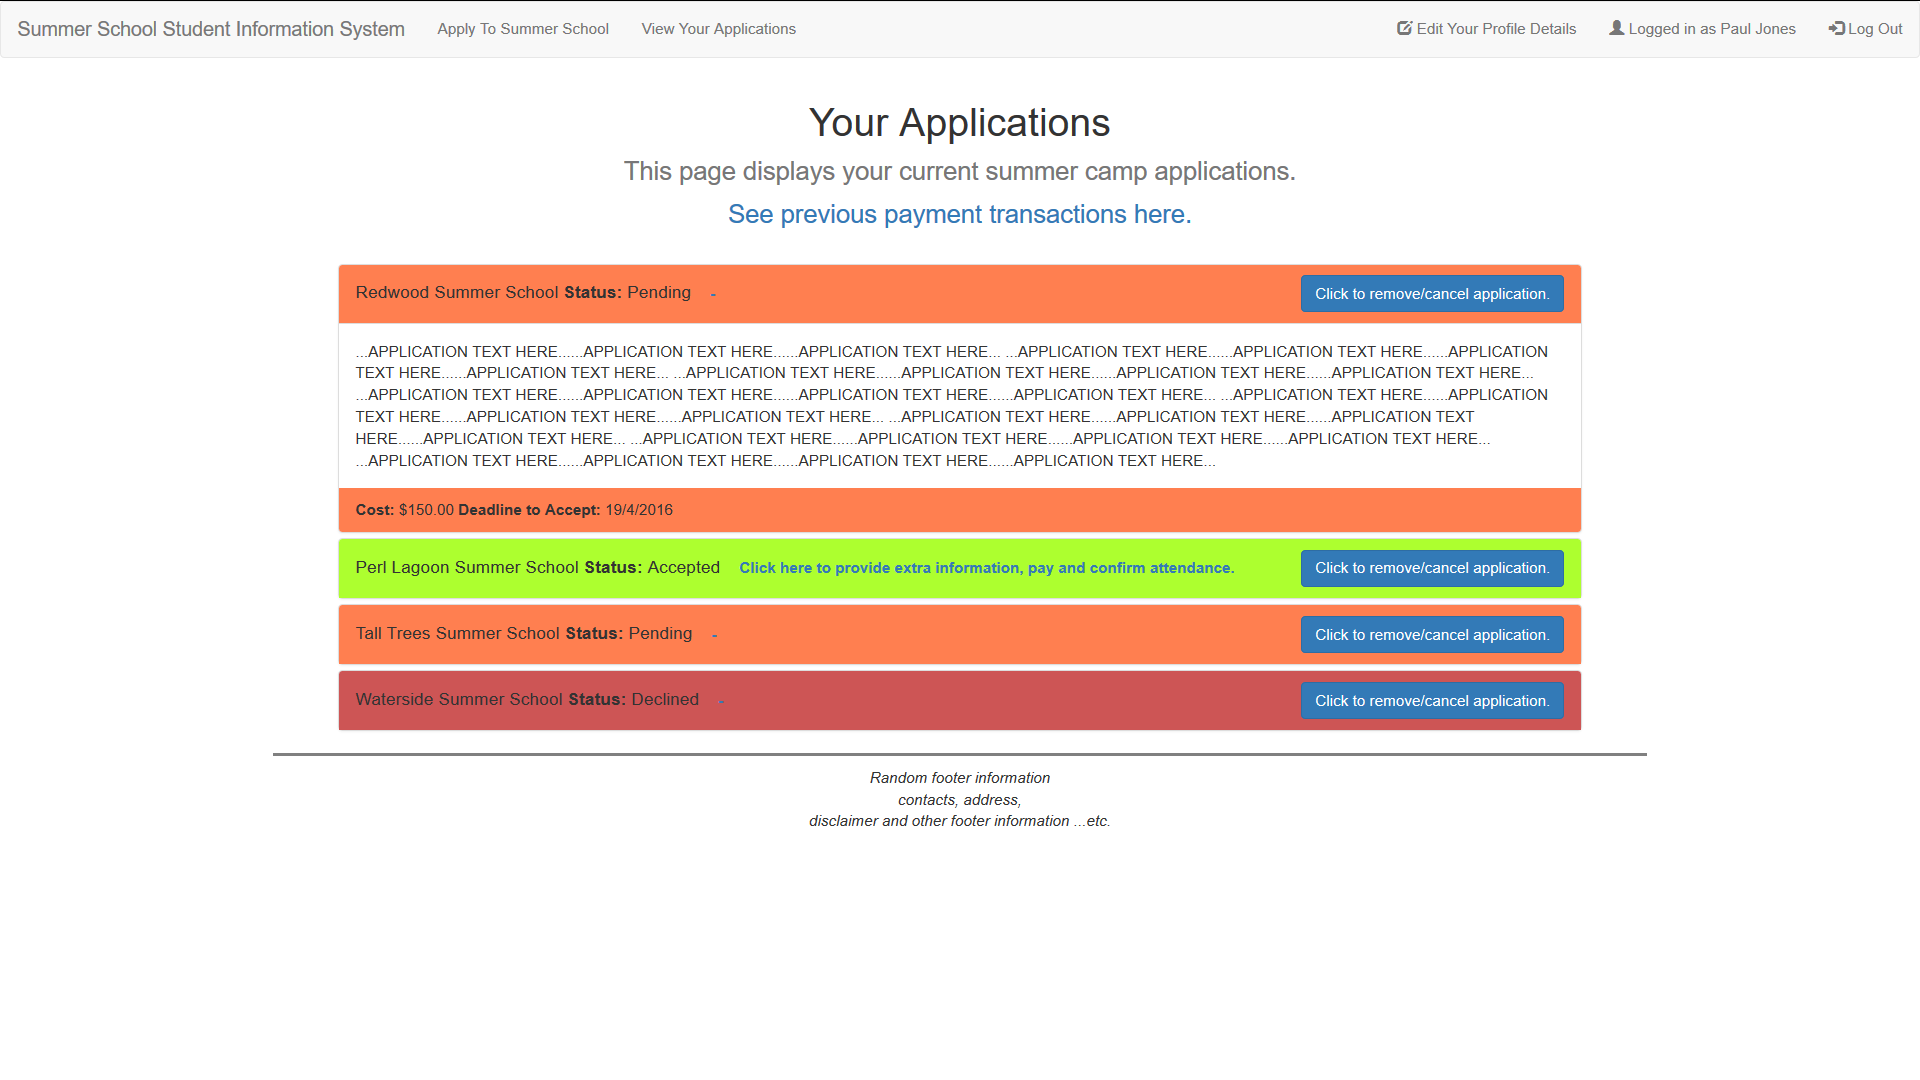
\includegraphics[width=\linewidth]{student-app2.png}
\caption{Student's Applications Page}
\label{fig:students-applications2}
\end{figure}
\begin{figure}[h]
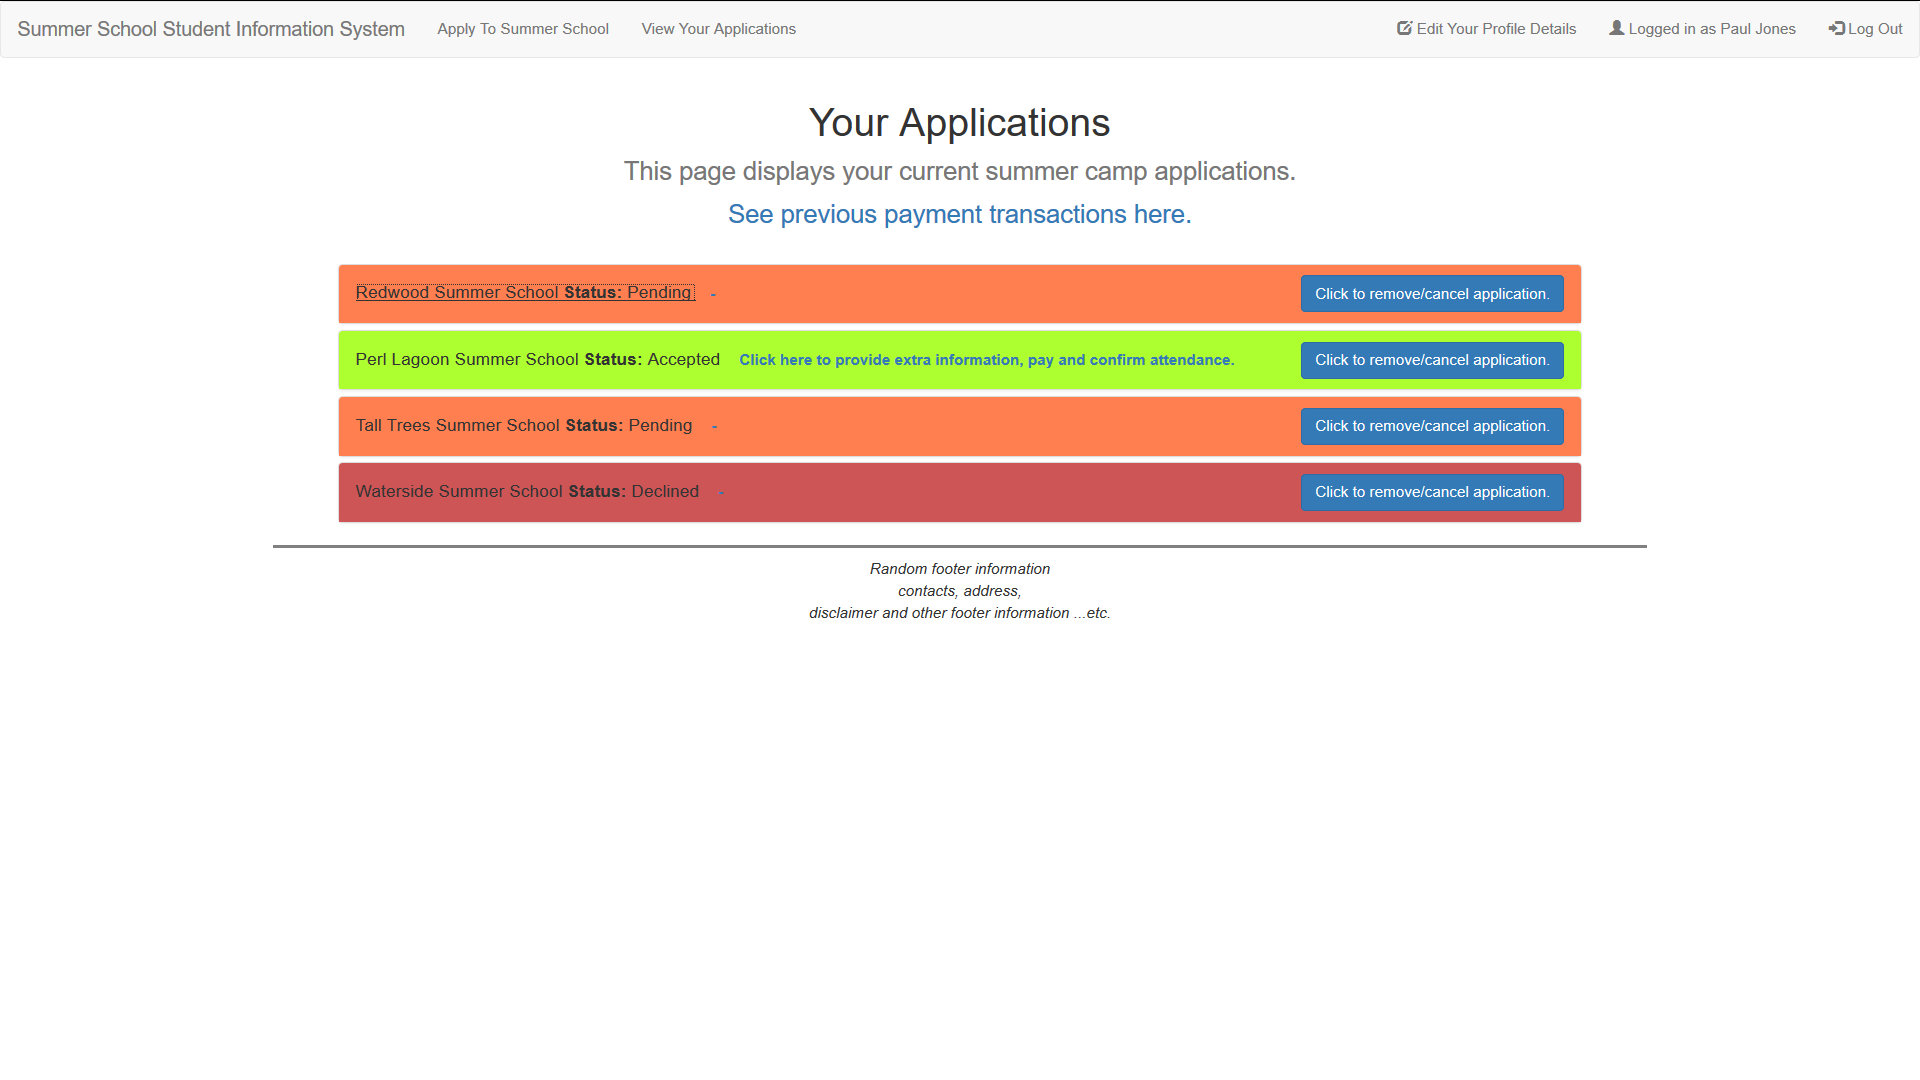
\includegraphics[width=\linewidth]{student-app3.png}
\caption{Student's Applications Page}
\label{fig:students-applications3}
\end{figure}
\begin{figure}[h]
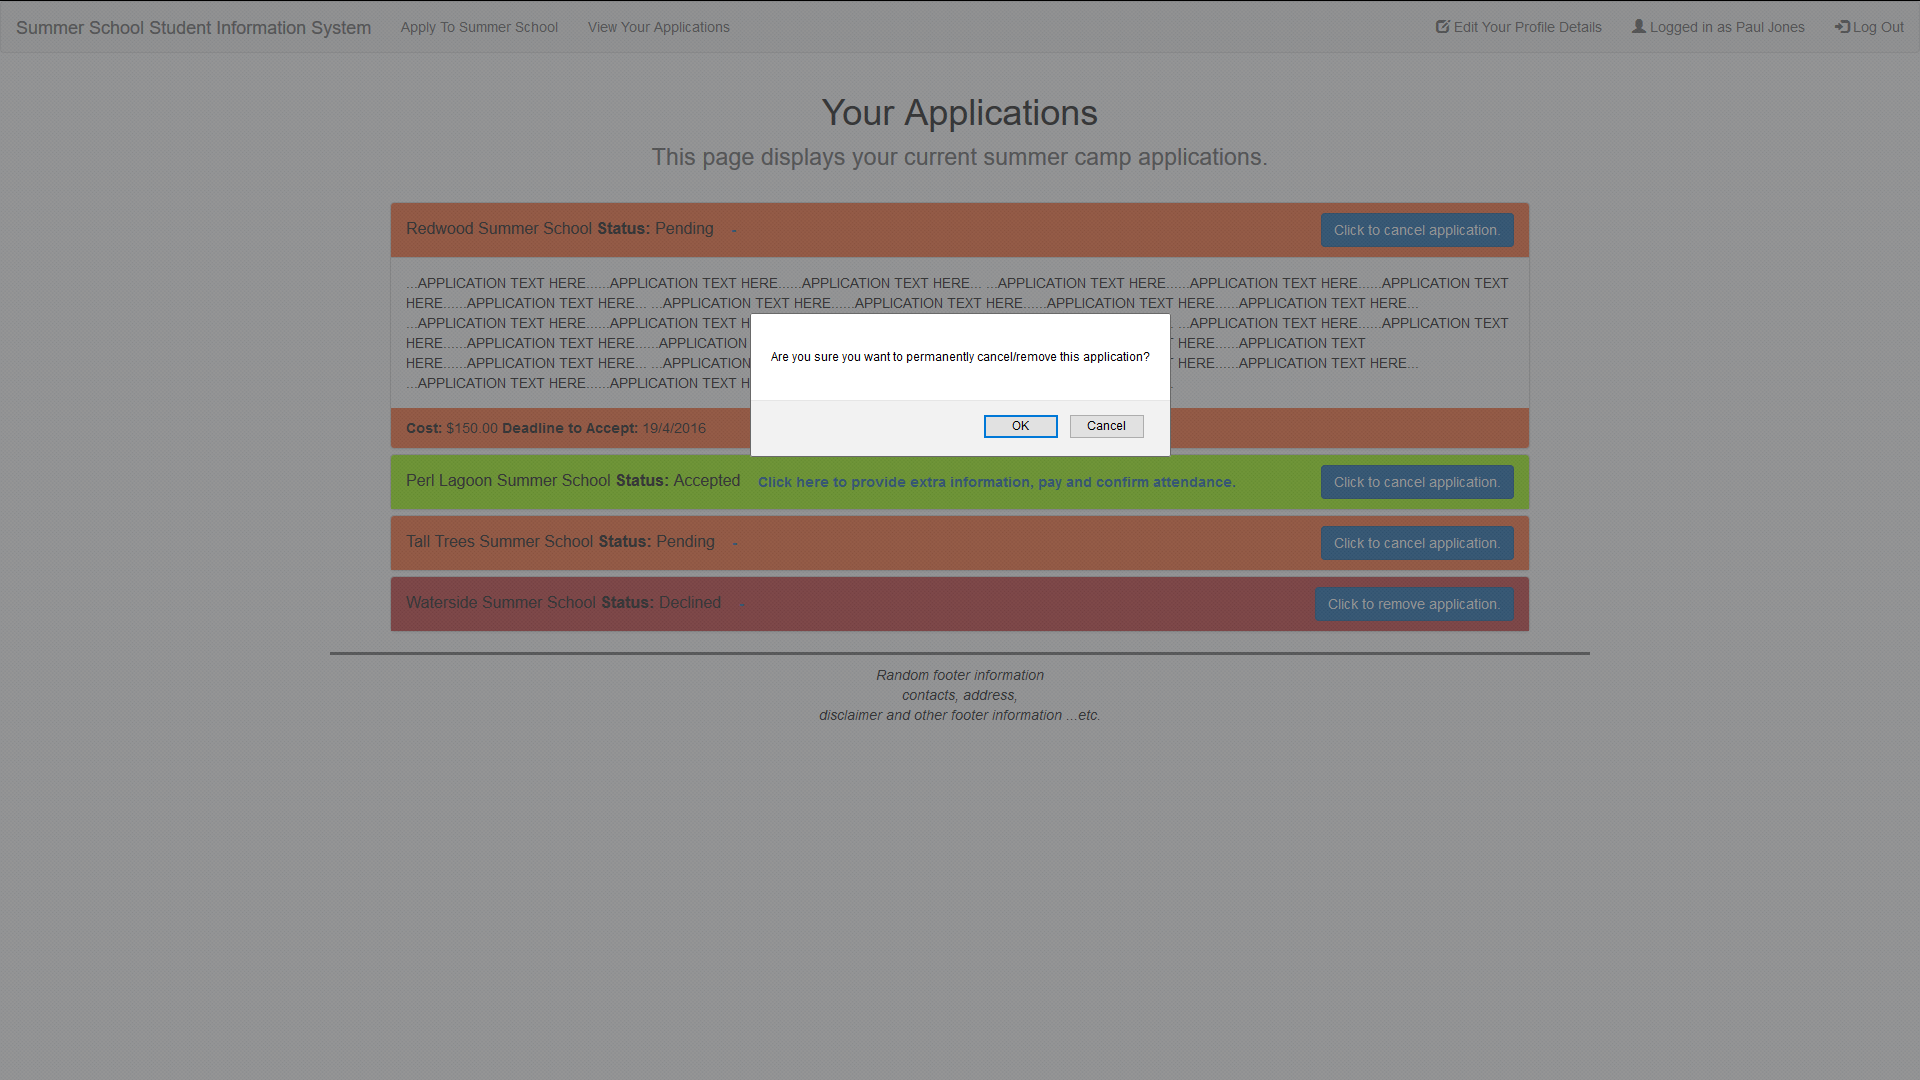
\includegraphics[width=\linewidth]{student-app-remove.png}
\caption{Student's Applications Page - When removing an application a confirm prompt will be shown.}
\label{fig:students-applications-remove}
\end{figure}
\begin{figure}[h]
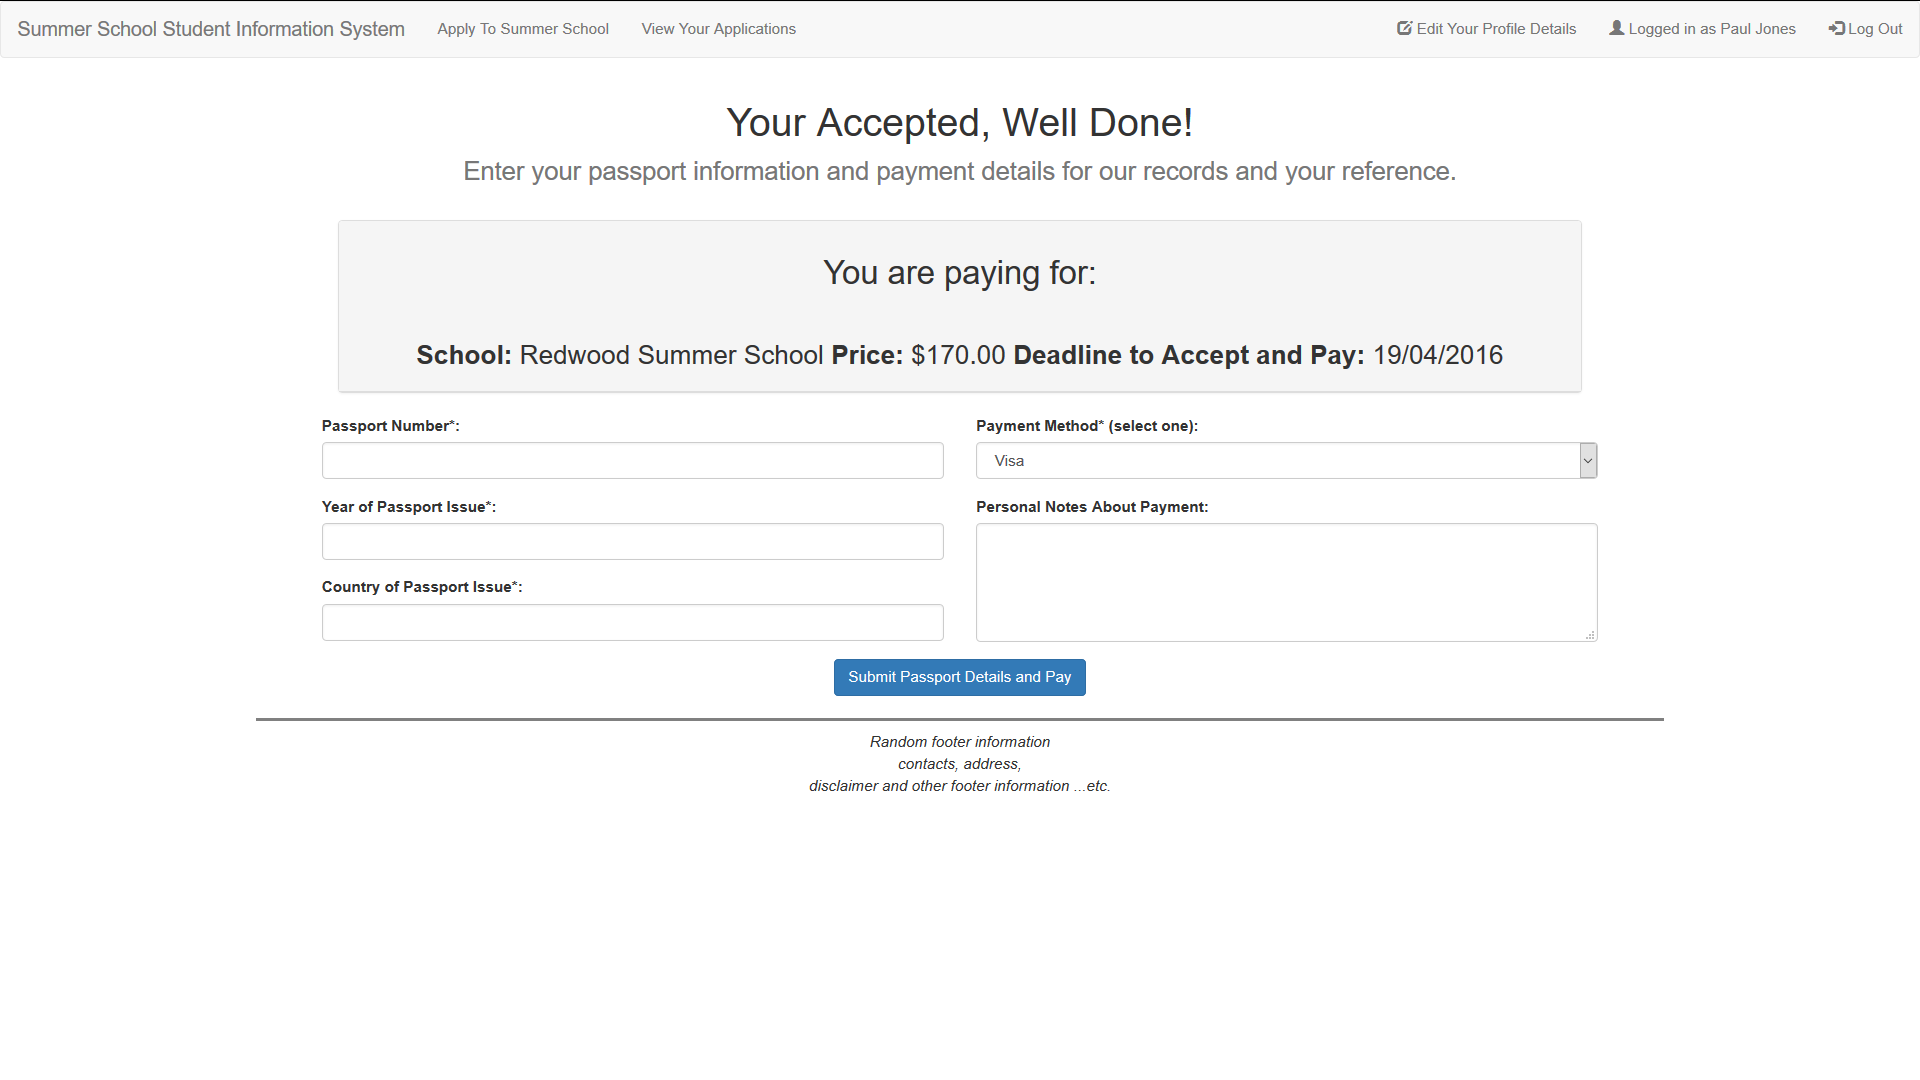
\includegraphics[width=\linewidth]{transaction.png}
\caption{Student Transaction Page}
\label{fig:student-transaction}
\end{figure}
\begin{figure}[h]
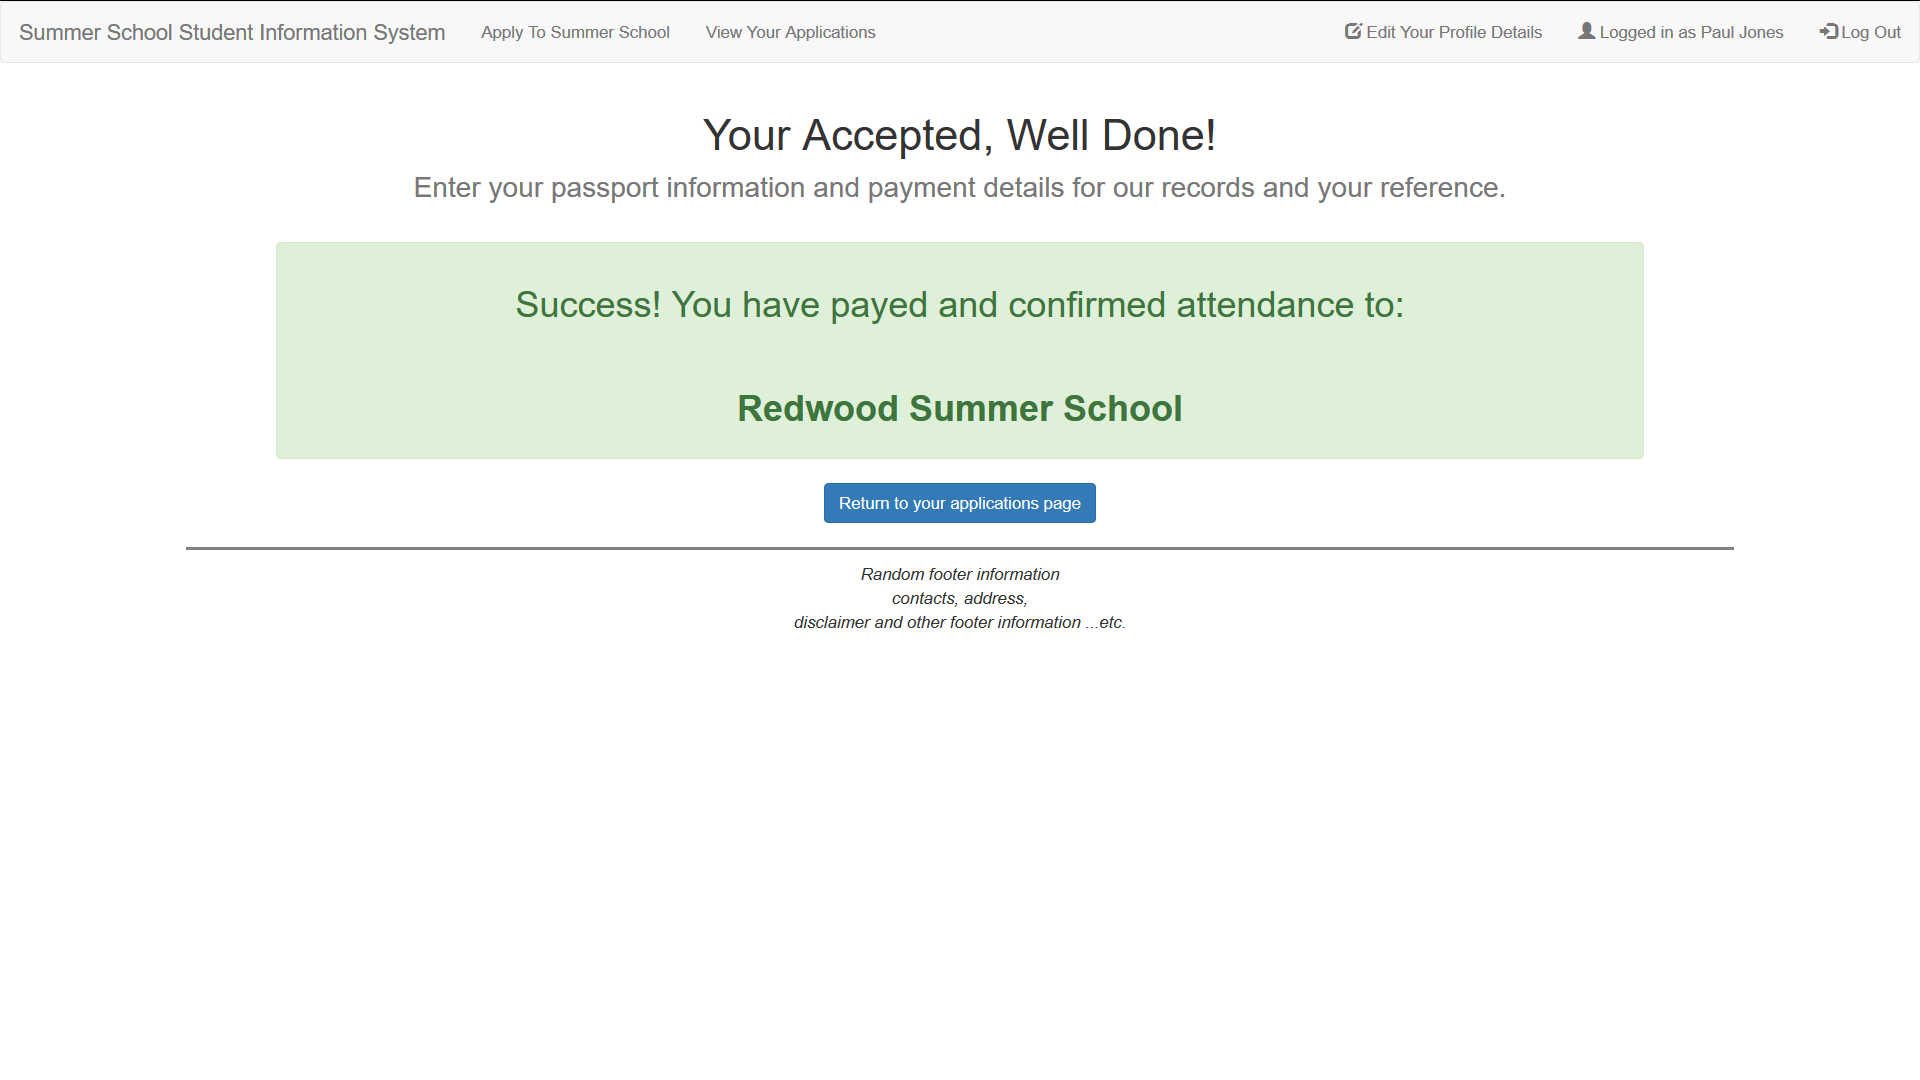
\includegraphics[width=\linewidth]{transaction-success.png}
\caption{Student Transaction Page - Success.}
\label{fig:student-transaction-success}
\end{figure}
\begin{figure}[h]
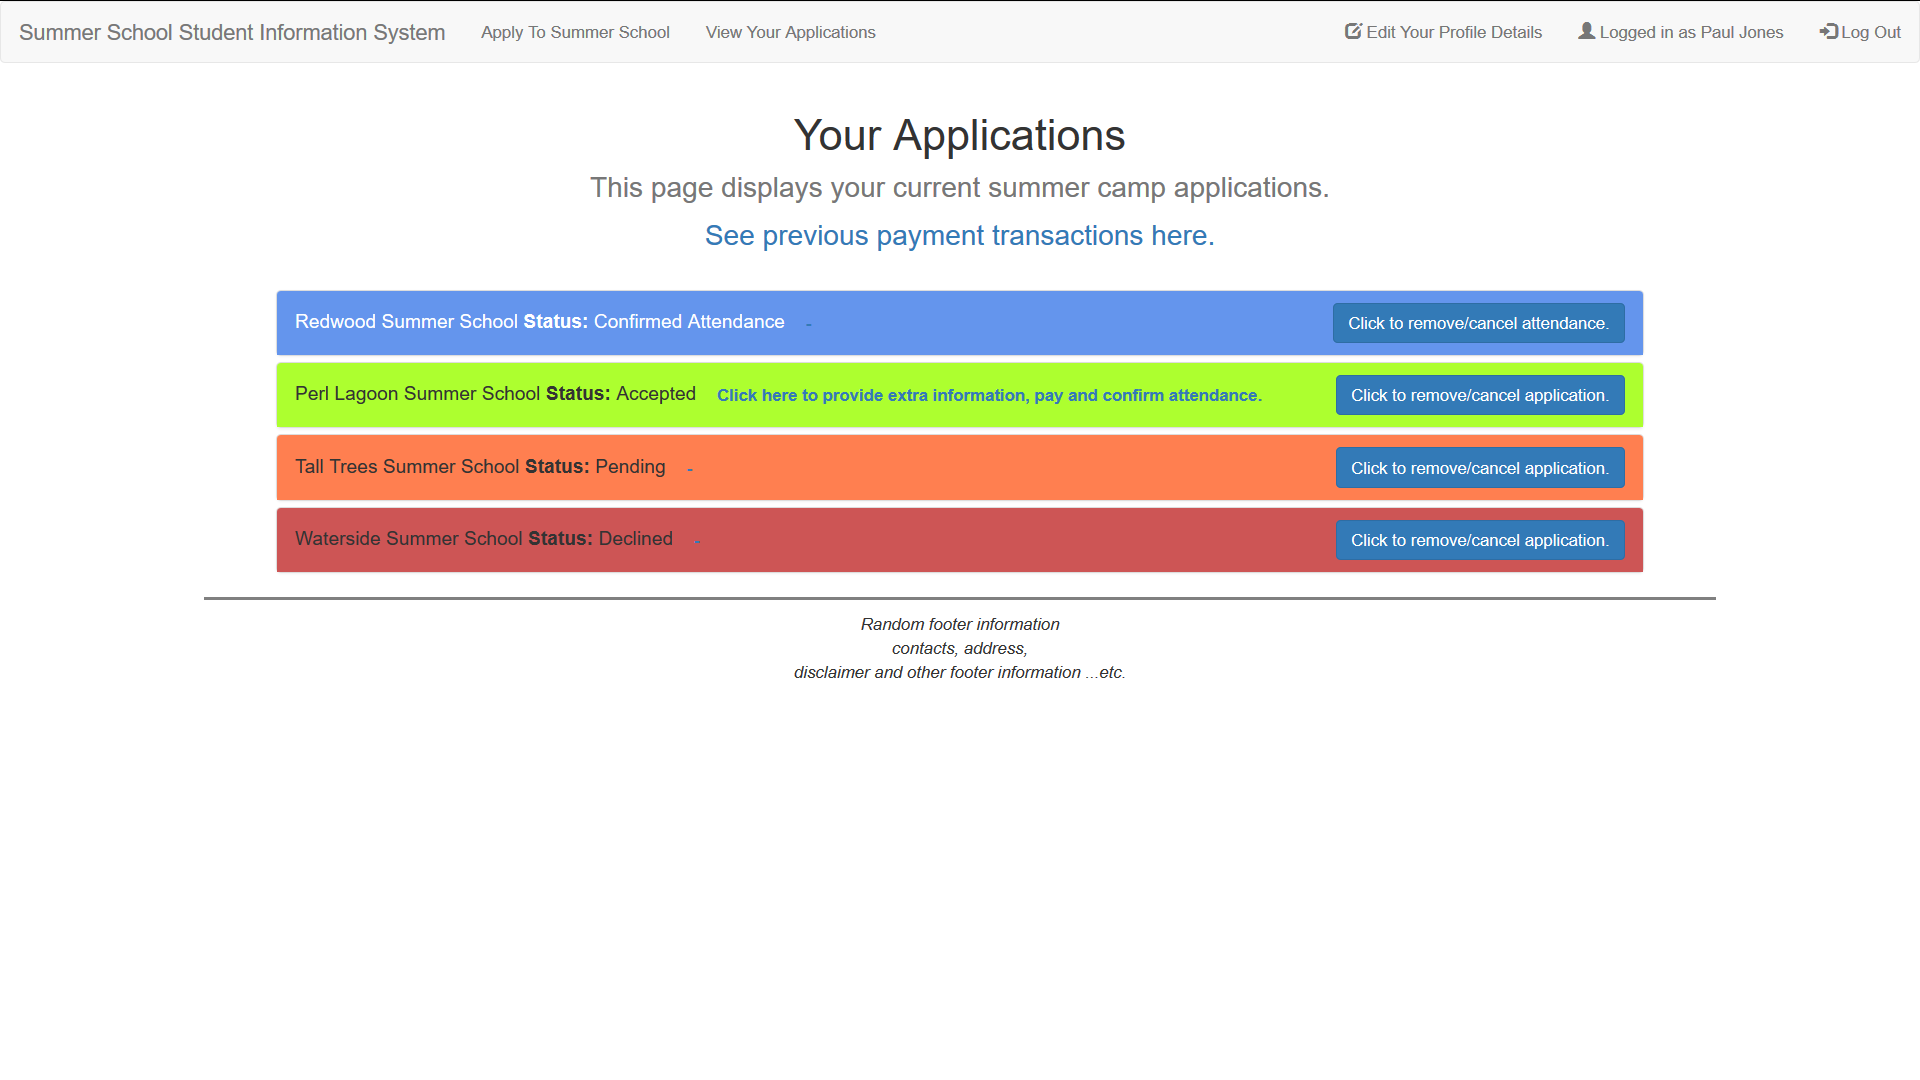
\includegraphics[width=\linewidth]{student-app-confirmed.png}
\caption{Student's Applications Page - Application is blue when a student has confirmed attendance to a school.}
\label{fig:students-applications-confirmed}
\end{figure}
\clearpage
\begin{figure}[H]
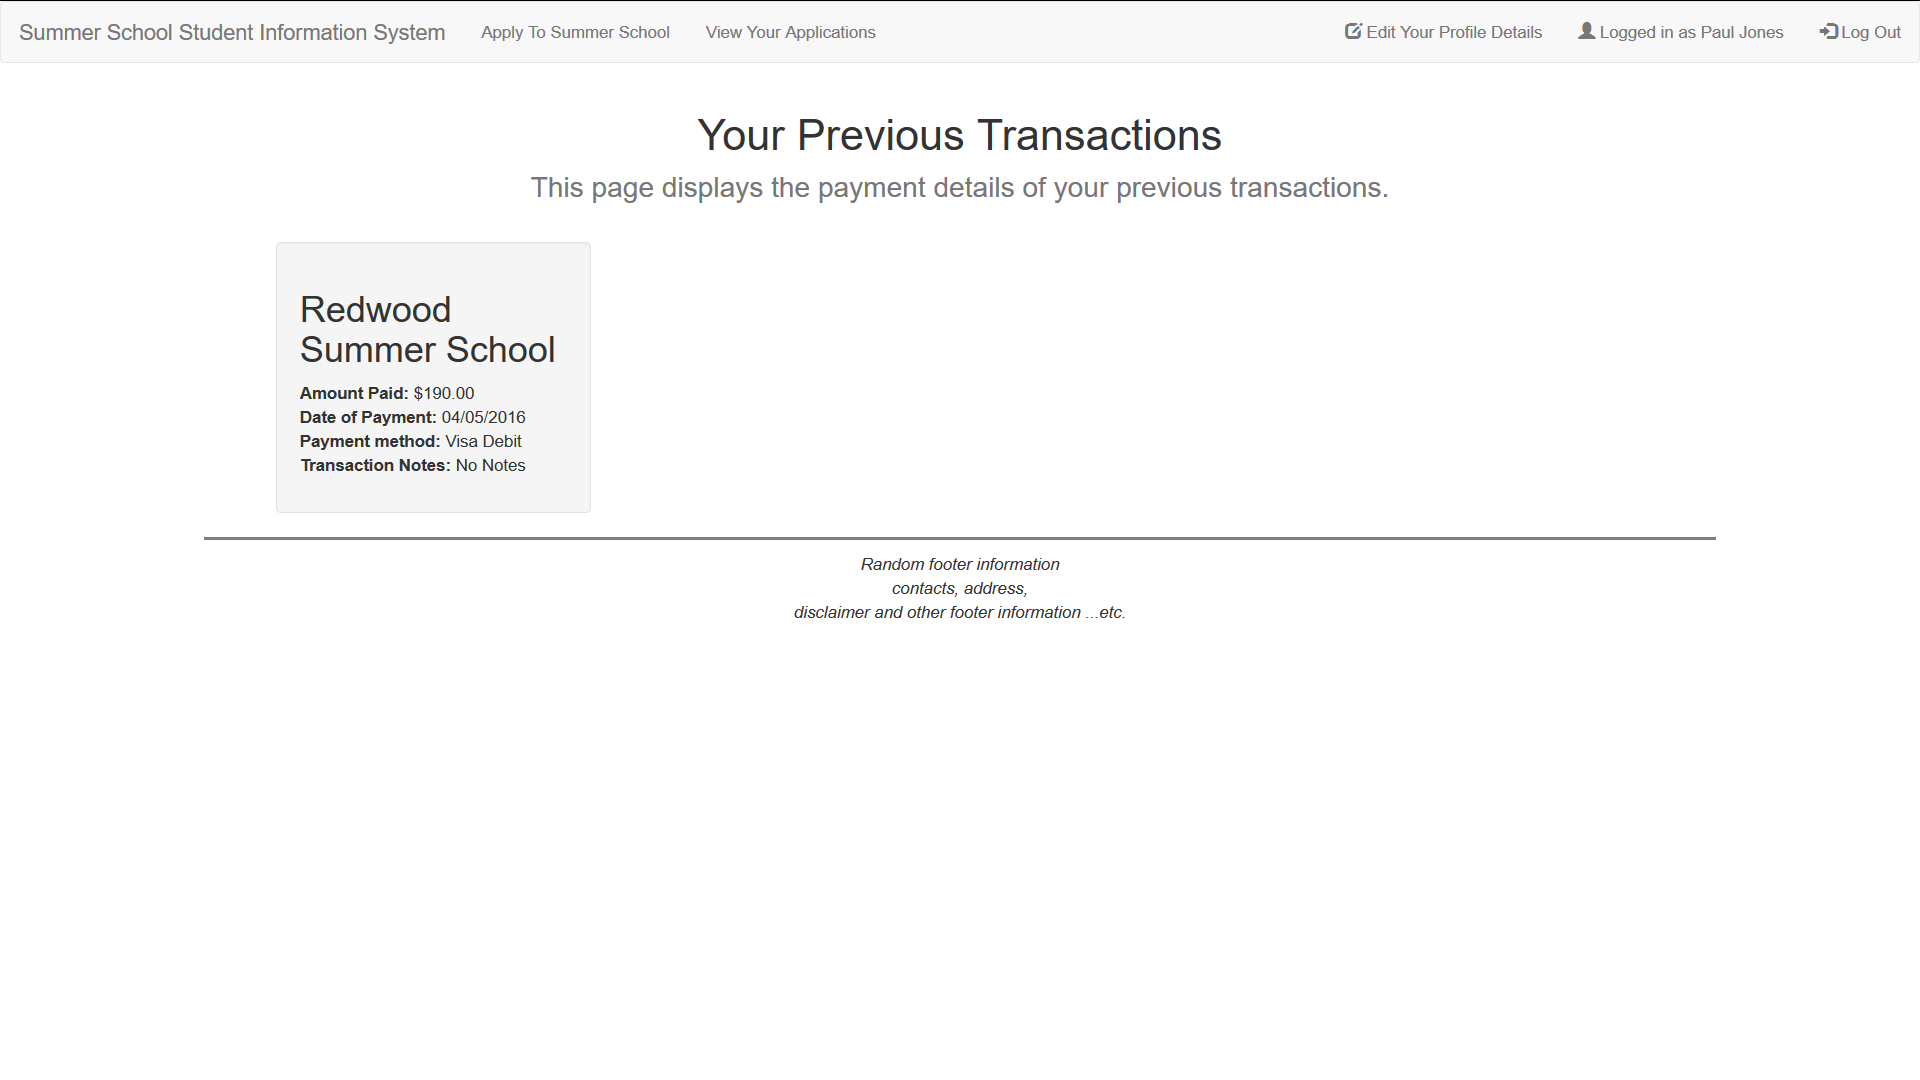
\includegraphics[width=\linewidth]{transaction-history.png}
\caption{Transaction History Page}
\label{fig:transaction-history}
\end{figure}
\begin{figure}[H]
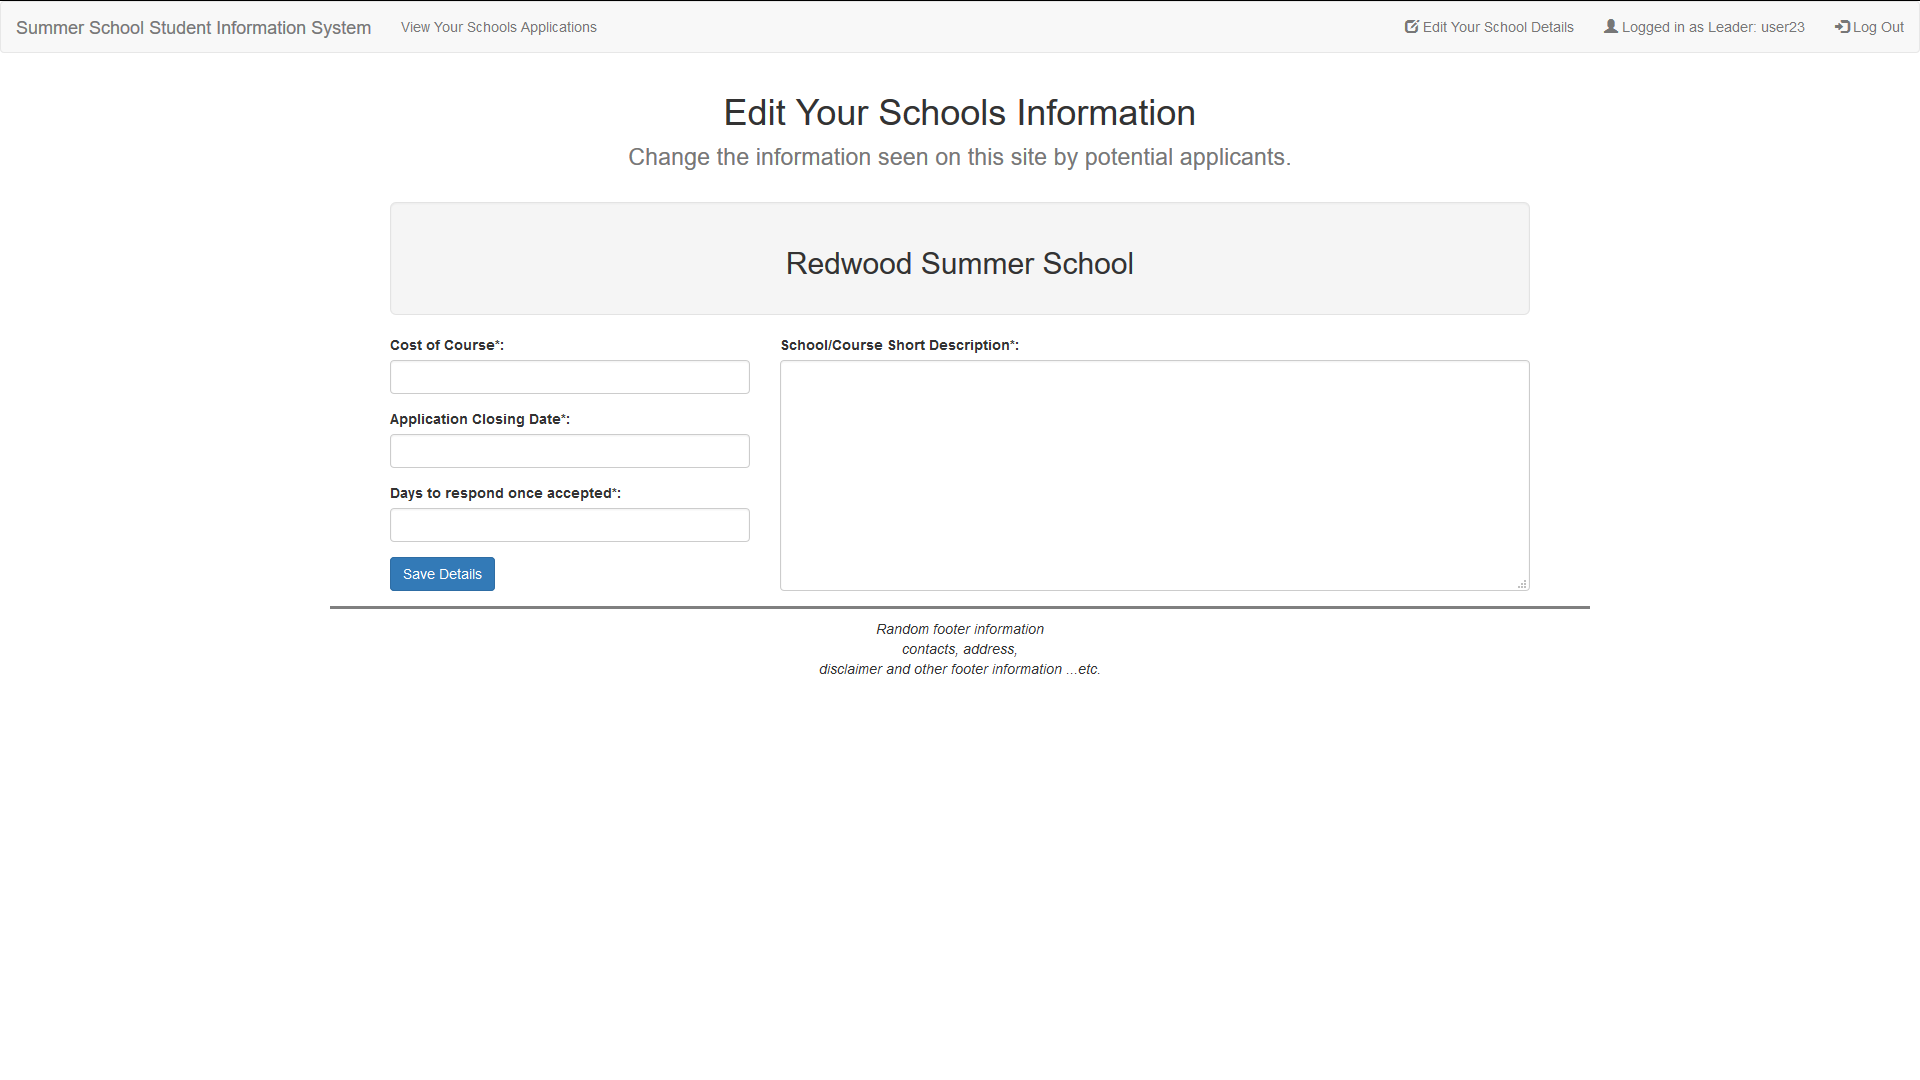
\includegraphics[width=\linewidth]{leader-profile.png}
\caption{School Profile Page}
\label{fig:school-profile}
\end{figure}
\begin{figure}[H]
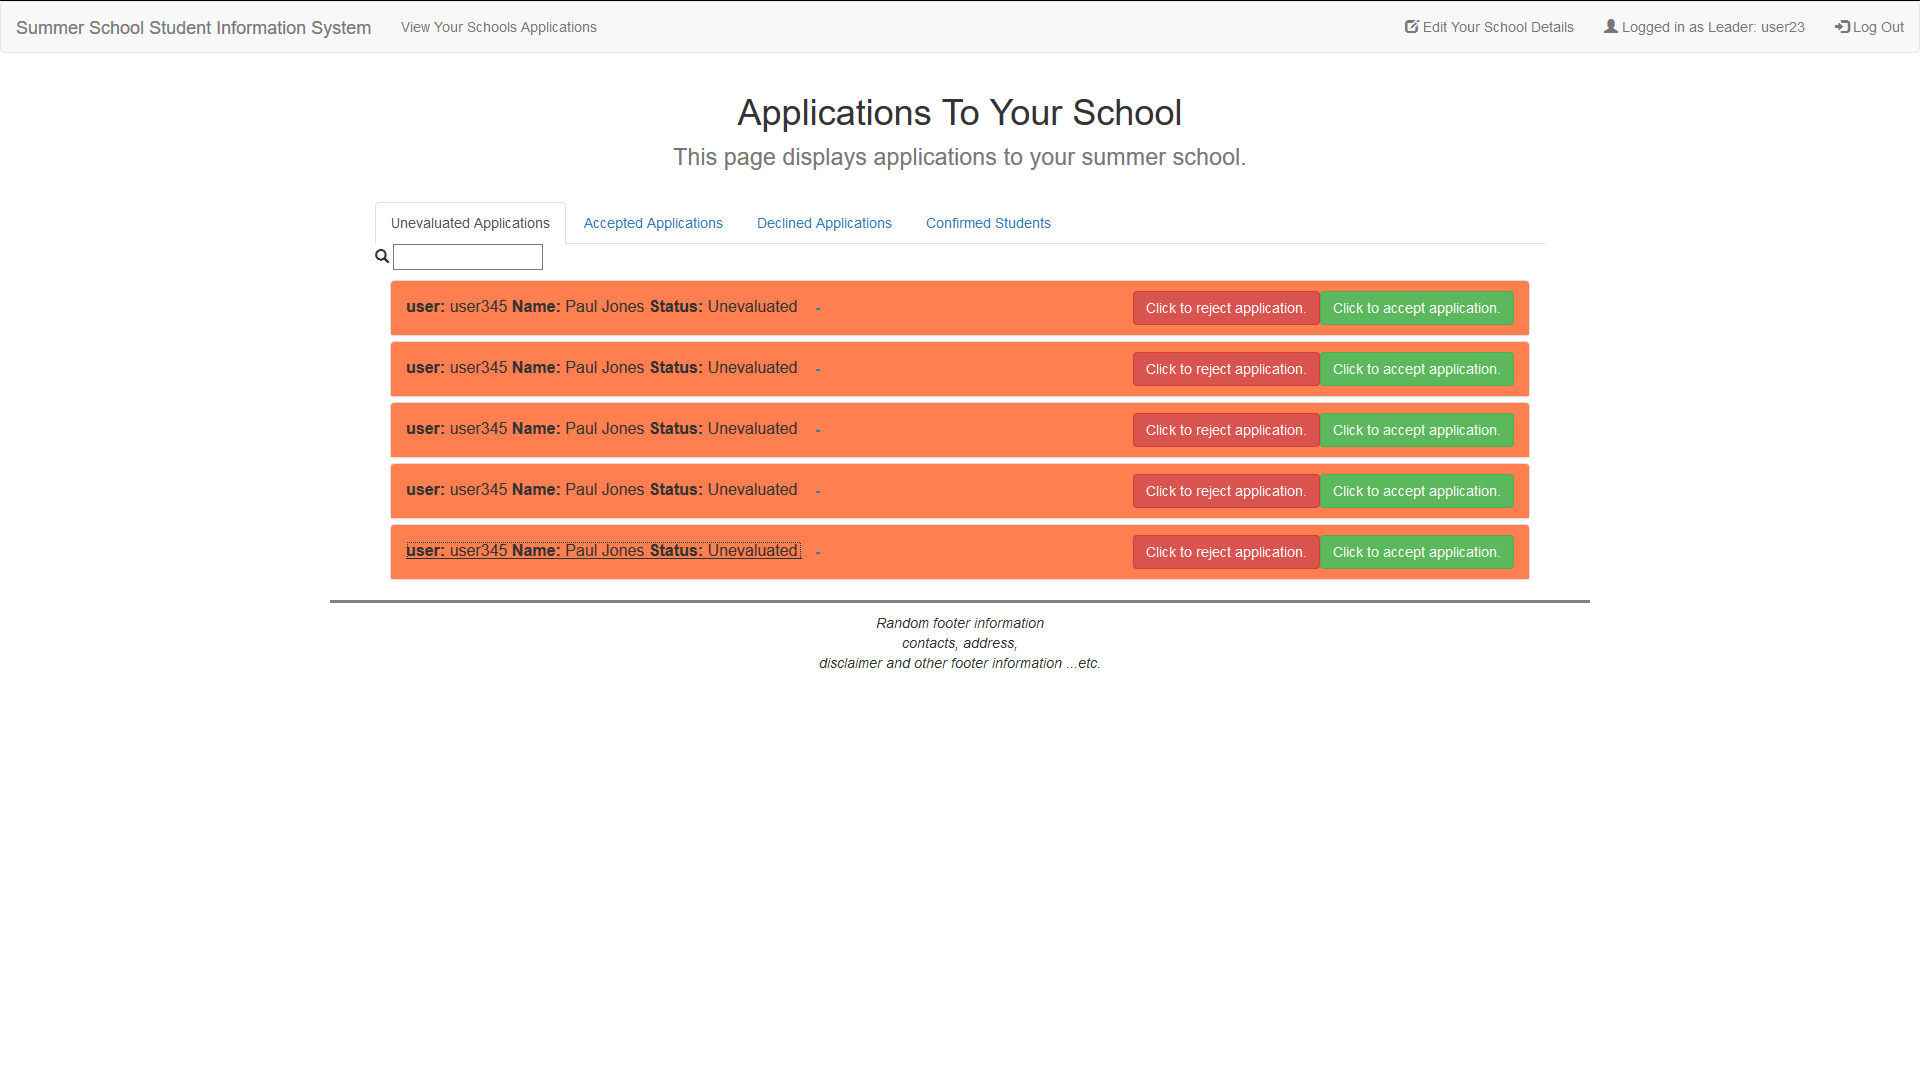
\includegraphics[width=\linewidth]{leader-app.png}
\caption{Leader's Applications Page}
\label{fig:leaders-applications}
\end{figure}
\begin{figure}[H]
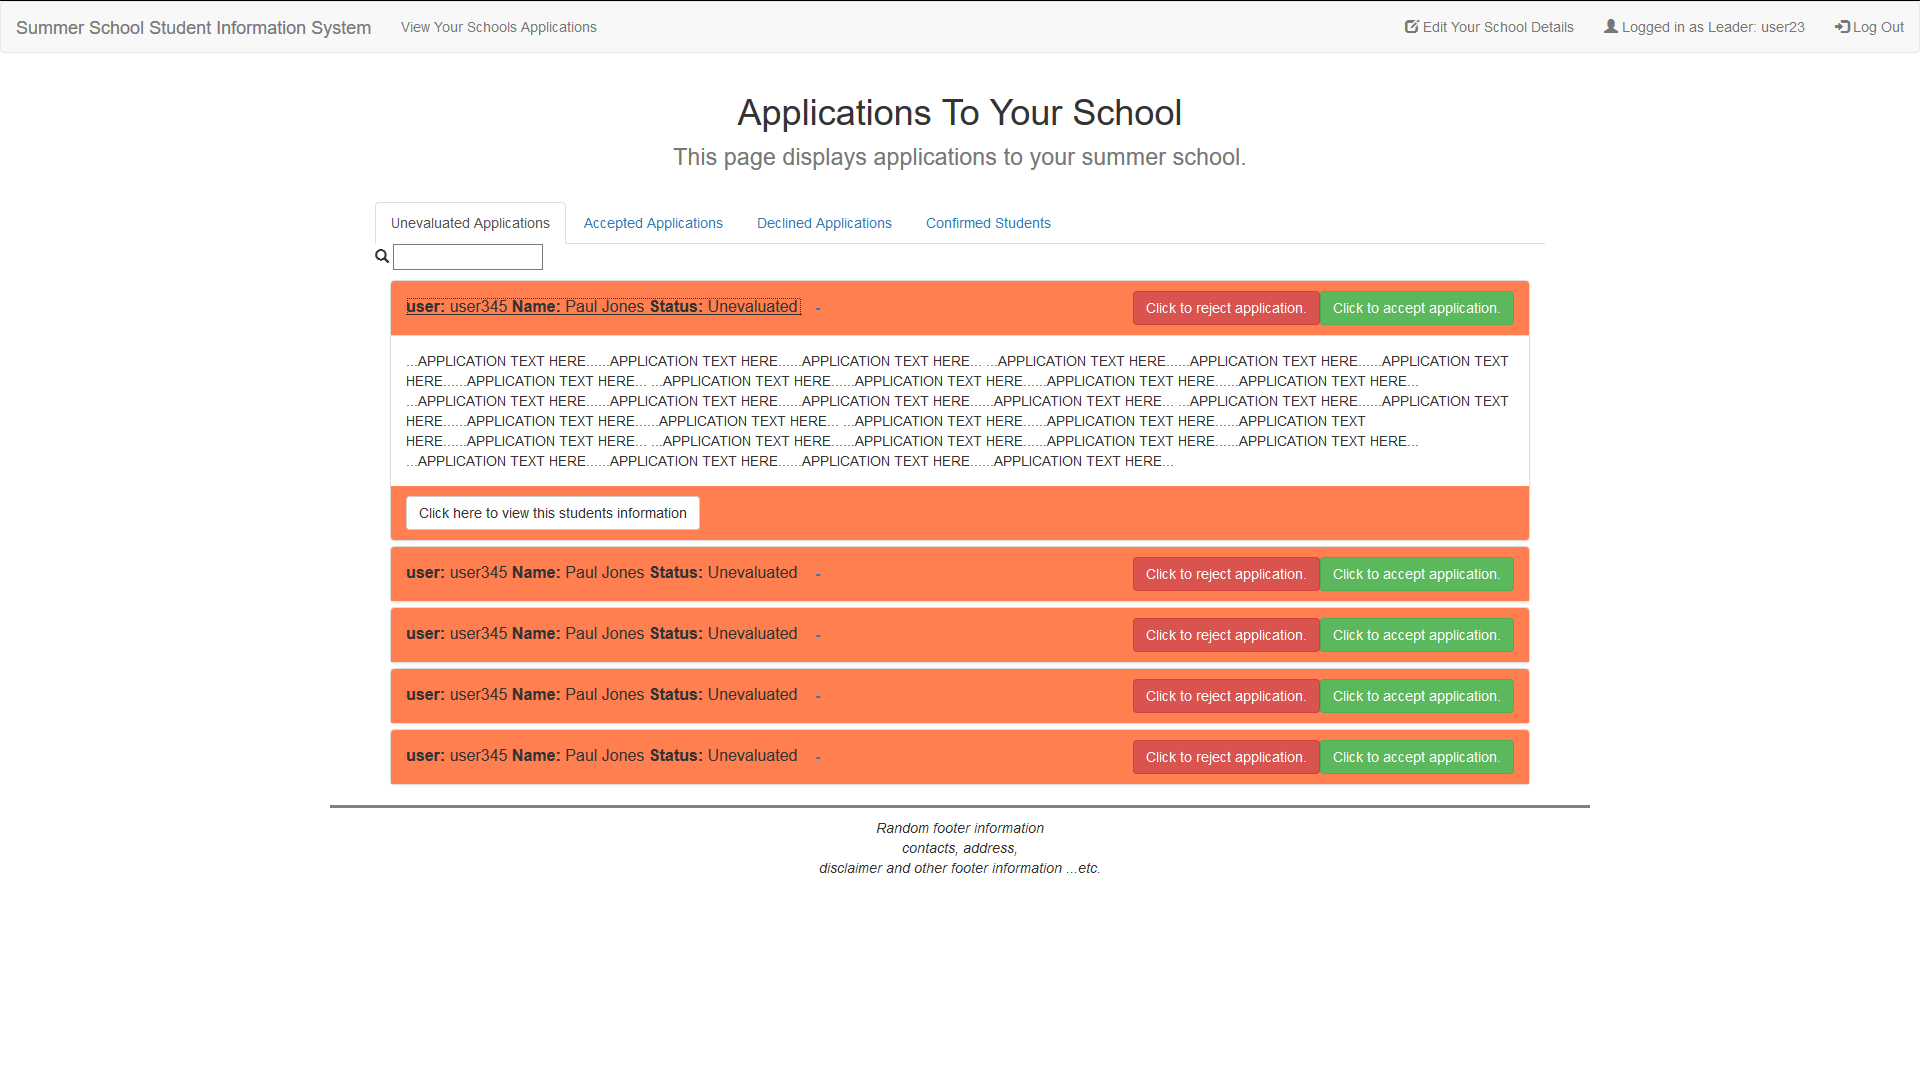
\includegraphics[width=\linewidth]{leader-app2.png}
\caption{Leader's Applications Page}
\label{fig:leaders-applications2}
\end{figure}
\clearpage
\subsection{Database design}
\begin{figure}[H]
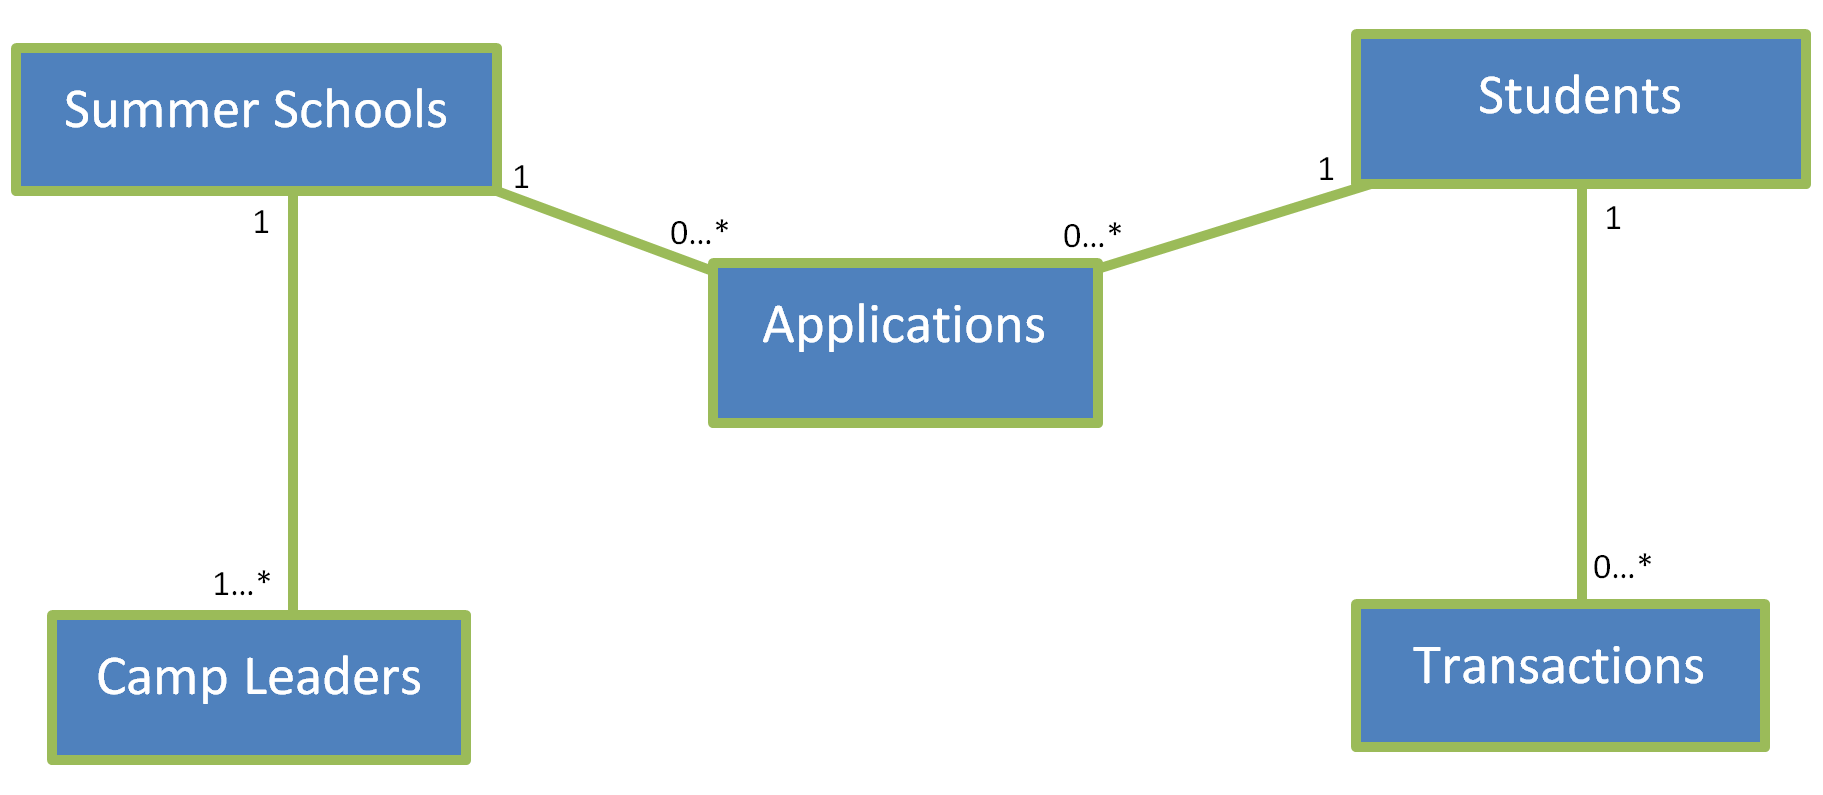
\includegraphics[width=\linewidth]{conceptualDatabase.png}
\caption{Conceptual Database Model.}
\label{fig:conceptual-database-model}
\end{figure}
\begin{figure}[H]
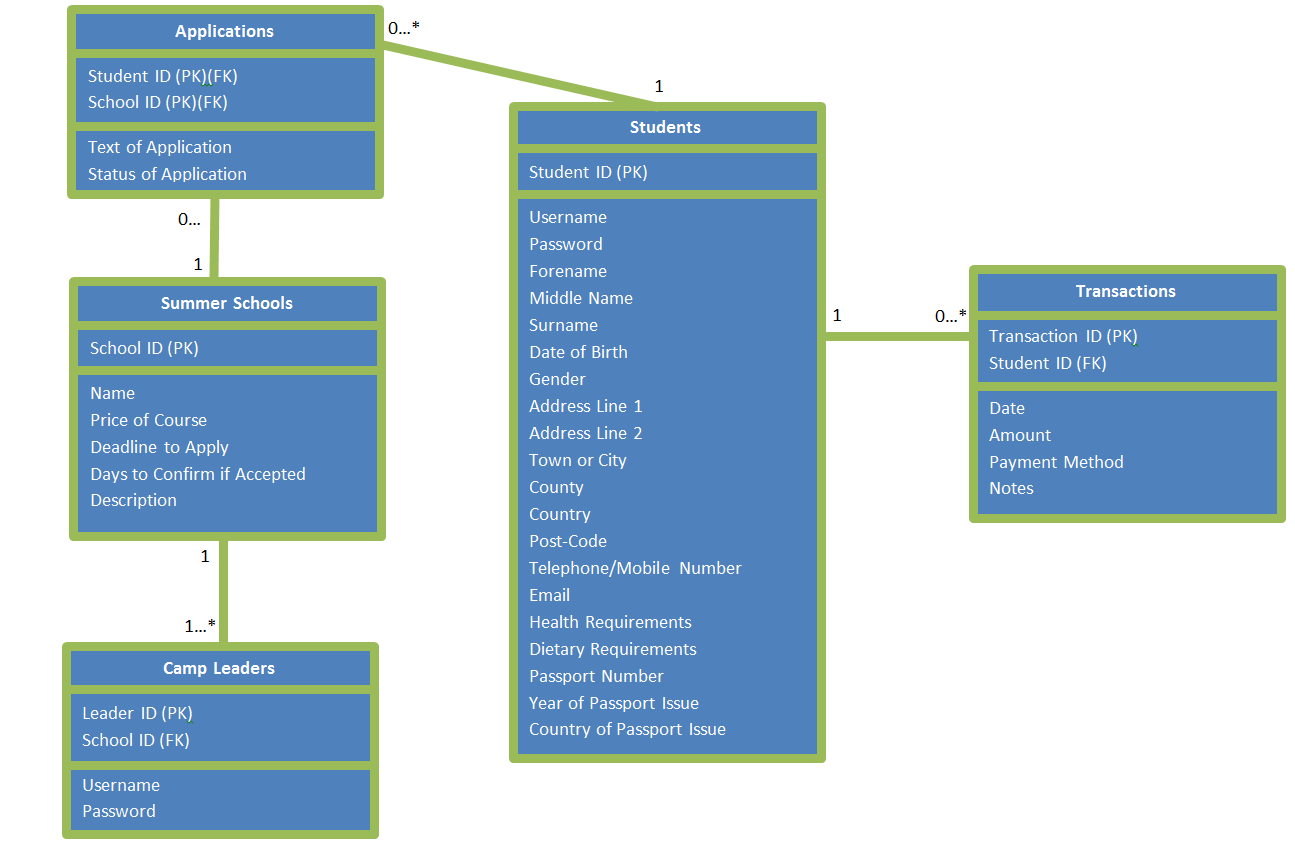
\includegraphics[width=\linewidth]{logicalDatabase.png}
\caption{Logical Database Model.}
\label{fig:logical-database-model}
\end{figure}
\begin{figure}[H]
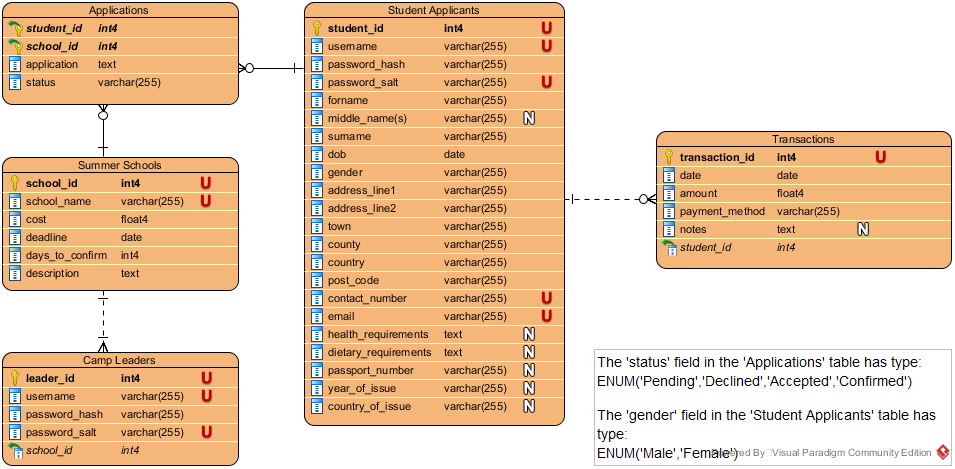
\includegraphics[width=\linewidth]{physicalDatabase.png}
\caption{Physical Database Model.}
\label{fig:physical-database-model}
\end{figure}
\label{thelastpage}
\end{document}
